% */ vim: set tw=150: */
\documentclass[11pt,a4paper]{article}
\pdfoutput=1

\usepackage{amsmath}
\usepackage[T1]{fontenc}

\usepackage{jheppub}
\usepackage{psfrag}
\usepackage{slashed}
\usepackage{cancel}
\usepackage{lscape}
\usepackage{caption}
\usepackage{array}
\usepackage{graphicx}
\usepackage{subcaption}
\usepackage{multirow}
\usepackage{tabularx}
\usepackage{makecell}
\usepackage[utf8]{inputenc}
\usepackage{amsmath}
\usepackage{amssymb}
\usepackage{relsize}
\usepackage{color}
\usepackage{slashed}
\usepackage{mathtools}
\usepackage{comment}
\usepackage{scalefnt}
\usepackage{siunitx}[=v2]
\sisetup{
    round-mode = off,
    round-precision = 4,
    scientific-notation = false,
    fixed-exponent = 0,
    group-digits = true,
    group-separator = {\,},
}

%{{{ macros

\renewcommand{\arraystretch}{1.3}

\definecolor{mypink}{RGB}{219, 48, 122}
\definecolor{mygreen}{rgb}{0,0.7,0}
\definecolor{raspberry}{rgb}{0.53,0.15,0.34}
\def\SB#1{\textcolor{mygreen}{{\bf\tt [SB: #1]}}}
\def\SZ#1{\textcolor{raspberry}{{\bf\tt [SZ: #1]}}}

%%% spinor products %%%

\def\zz{\boldsymbol{Z}}
\def\mi{\mathrm{MI}}
\def\cF{\mathcal{F}}
\def\cP{\mathcal{P}}
\def\cC{\mathcal{C}}
\def\cA{\mathcal{A}}
\def\cN{\mathcal{N}}
\def\cO{\mathcal{O}}
\def\cD{\mathcal{D}}
\def\cQ{\mathcal{Q}}
\def\cJ{\mathcal{J}}
\def\cI{\mathcal{I}}
\def\cT{\mathcal{T}}
\def\nn{\nonumber \\ }

\def\la{\langle}
\def\ra{\rangle}
\def\spA#1#2{\la#1#2\ra}
\def\spB#1#2{[#1#2]}
\def\spAB#1#2#3{\la#1|#2|#3]}
\def\spBA#1#2#3{[#1|#2|#3\ra}
\def\spAA#1#2#3{\la#1|#2|#3\ra}
\def\spBB#1#2#3{[#1|#2|#3]}
\def\spab#1#2{\la#1|#2]}
\def\spaa#1#2#3#4{\la#1|#2|#3|#4\ra}
\def\spbb#1#2#3#4{[#1|#2|#3|#4]}
\def\wh#1{\widehat#1}
\DeclareMathOperator{\tr}{\rm tr}
\def\trm{\tr_-}
\def\trp{\tr_+}
\def\MP#1#2{(#1\cdot#2)}
\def\trfive{\tr_5}
\def\spAXB#1#2#3#4#5{\la#1|#2|#3|#4|#5]}

\def\bra#1{\langle #1|}
\def\ket#1{|#1 \rangle}
\def\sqbra#1{[#1|}
\def\sqket#1{|#1]}
\def\braket#1{\langle #1 \rangle}

\def\eps{\epsilon}
\def\fl#1{#1^\flat}
\def\tl#1{\tilde{#1}}
\def\wh{\widehat}
\def\tC{\tilde{C}}
\def\qb{{\bar{q}}}
\def\sb{\bar{s}}
\def\Sb{\bar{S}}
\def\lb{\bar{\ell}}
\def\tb{{\bar{t}}}
\def\ttgg{\bar{t}tgg}
\def\mren{\mathrm{mren}}
\def\ren{\mathrm{ren}}
\def\mct{\mathrm{mct}}
\def\ceps{C_\eps}
\def\as{\alpha_s}
\def\dk#1{\frac{d^d k_{#1}}{i\pi^{d/2}e^{-\eps \gamma_E}}}

\def\e{\epsilon}
\def\tT{\tilde{T}}
\def\coll#1#2{\overset{#1||#2}{\to}}
\def\inf{{\rm Inf}}
\def\gg#1{\gamma_{#1}}
\def\XX{\chi}

\def\cv#1#2{\AB{#1}{\gamma^\mu}{#2}}
\def\cvS#1#2#3{\AB{#1}{#2}{#3}}

\def\MHVb{$\overline{\rm MHV}$}
\def\boxX{$\xcancel{\rm\bf box}$}

\def\fl#1{{#1^{\flat}}}
\def\flm#1{{#1^{\flat,\mu}}}
\def\kf#1{{\fl{K_{#1}}}}
\def\kfm#1{{\flm{K_{#1}}}}

\def\ulim#1{\underset{#1}{\lim}}

\def\fbox#1{F^{(#1)}_{\mathrm{box}}}
\def\lh{\hat{L}}
\def\li#1{\mathrm{Li}_{#1}}

\def\finr{{\mathcal{F}}}
\def\pole{{\mathcal{P}}}
\def\cusp{{\mathrm{cusp}}}

\newcommand{\njet}{\texttt{NJet}}
\newcommand{\pentagonfunctions}{\texttt{PentagonFunctions++}}
\newcommand{\finiteflow}{\texttt{FiniteFlow}}
\newcommand{\qd}{\texttt{QD}}
\newcommand{\eigen}{\texttt{Eigen}}
\newcommand{\nnlojet}{\texttt{NNLOJET}}
\newcommand{\mathematica}{\texttt{Mathematica}}
\newcommand{\form}{\texttt{FORM}}
\newcommand{\qgraf}{\texttt{QGRAF}}
\newcommand{\spinney}{\texttt{Spinney}}
\newcommand{\cpp}{\texttt{C++}}

%%Christian's command
\newcommand{\eqcite}[1]{(\ref{#1})}
\newcommand{\dd}{\mathop{}\!\mathrm{d}}

\newcommand{\fp}{\texttt{f64}}
\newcommand{\fpp}{\texttt{f128}}
\newcommand{\fppp}{\texttt{f256}}

%%%% typesetting equations %%%%
\def\s#1{s_{#1}}
\def\d#1#2{#1\cdot #2}
\def\p#1{#1}
\def\pp#1{p_{#1}}
\def\f#1{#1^\flat}
\def\n#1{\eta_{#1}}

\def\Adcc{B_n^{(1)}}

\def\usepic#1#2{\parbox{#1}{\includegraphics[width=#1]{#2}}}
\def\usepix#1#2#3#4#5#6{\parbox{#1}{\includegraphics[width=#1,trim= #3 #4 #5 #6,clip=true]{#2}}}

\def\hpl11{{\mathrm{HPL}}_{1,1}}

\newcolumntype{C}[1]{>{\hsize=#1\hsize\centering\arraybackslash}X}%

\newcolumntype{Z}{r<{\hspace{3mm}}}
\newcommand\mc[2]{\multicolumn{1}{>{\centering}p{#2}}{#1}} % handy shortcut macro
% }}}

%%\allowdisplaybreaks

\newcommand{\MSbar}{\ensuremath{\overline{\text{MS}}}}
\newcommand{\fonll}{FONLL}
\newcommand{\nlonnllpart}{NLO+NNLL\textsubscript{part}+$y_by_t$}
\newcommand{\nnnres}{$\text{N}^3\text{LL'}+\text{aN}^3\text{LO}$}

\providecommand{\href}[2]{#2}

\newcommand{\incl}{{\tt inclusive}}
\newcommand{\fidYR}{{\tt fiducial-YR}}
\newcommand{\fidATLAS}{{\tt fiducial-ATLAS}}

\newcommand{\stepone}{{Step\,I}}
\newcommand{\steptwo}{{Step\,II}}
\newcommand{\stepthree}{{Step\,III}}

\newcommand\tS{\tilde{S}}
\newcommand\F{${\textrm F}$}
\newcommand\FJ{${\textrm FJ}$}
\newcommand\FJJ{${\textrm FJJ}$}
\newcommand\PhiBorn{\Phi_{\scriptscriptstyle \textrm B}}
\newcommand\PhiReal{\Phi_{\scriptscriptstyle \textrm R}}
%\newcommand\PhiB{\Phi_{\scriptscriptstyle \textrm H}}
\newcommand\PhiB{\Phi_{\scriptscriptstyle \textrm F}}
\newcommand\PhiBres{\Phi_{\scriptscriptstyle \textrm F,res}}

\newcommand{\flav}{\ell}
\newcommand{\flavBorn}{\flav_{\scriptscriptstyle \textrm B}}
\newcommand{\fullflavBorn}{\hat \flav_{\scriptscriptstyle \textrm B}}
\newcommand{\flavprimeBorn}{\flav'_{\scriptscriptstyle \textrm B}}
\newcommand{\fullflavprimeBorn}{\hat \flav'_{\scriptscriptstyle \textrm B}}
\newcommand{\flavB}{\flav_{\scriptscriptstyle \textrm F}}
\newcommand{\fullflavB}{\hat \flav_{\scriptscriptstyle \textrm F}}
\newcommand{\flavBJ}{\flav_{\scriptscriptstyle \textrm FJ}}
\newcommand{\fullflavBJ}{\hat \flav_{\scriptscriptstyle \textrm FJ}}
\newcommand{\flavBJJ}{\flav_{\scriptscriptstyle \textrm FJJ}}
\newcommand{\fullflavBJJ}{\hat \flav_{\scriptscriptstyle \textrm FJJ}}
\newcommand{\projflav}{\flavB\leftarrow\flavBJ}
\newcommand{\CF}{C_{\mathrm{F}}}
\newcommand{\CA}{C_{\mathrm{A}}}
\newcommand{\NC}{N_{\mathrm{c}}}
\newcommand{\nf}{N_f}
\newcommand{\TF}{T_{\mathrm{F}}}

\newcommand{\flavZg}{\flav_{\scriptscriptstyle Z\gamma}}
\newcommand{\fullflavZg}{\hat \flav_{\scriptscriptstyle Z\gamma}}
\newcommand{\flavZgJ}{\flav_{\scriptscriptstyle Z\gamma {\textrm J}}}
\newcommand{\fullflavZgJ}{\hat \flav_{\scriptscriptstyle Z\gamma {\textrm J}}}
\newcommand{\flavZgJJ}{\flav_{\scriptscriptstyle Z\gamma {\textrm J}}}
\newcommand{\fullflavZgJJ}{\hat \flav_{\scriptscriptstyle Z\gamma {\textrm J}}}
\newcommand{\projflavZg}{\flavZg\leftarrow\flavZgJ}

%\newcommand\PhiBJ{\Phi_{\scriptscriptstyle \textrm HJ}}
\newcommand\PhiBJ{\Phi_{\scriptscriptstyle \textrm FJ}}
\newcommand\ZJ{Z\gamma J}
\newcommand\PhiZJ{\Phi_{\scriptscriptstyle \textrm Z\gamma J}}
\newcommand\PhiBJbar{{\bar \Phi}'_{\scriptscriptstyle \textrm FJ}}
\newcommand\PhiBJJ{\Phi_{\scriptscriptstyle \textrm FJJ}}
\newcommand\PhiZJJ{\Phi_{\scriptscriptstyle \textrm Z\gamma JJ}}
\newcommand\PhiZgam{\Phi_{\scriptscriptstyle \textrm Z\gamma}}
\newcommand{\Fcorr}{F^{\tmop{corr}}_\ell}
\newcommand{\order}[1]{{\cal O}\left(#1\right)}
\newcommand{\aew}{\alpha_{\text{\scalefont{0.77}EW}}} 
\newcommand{\aw}{\alpha_w}
\newcommand{\asCMW}{\alpha_s^{\textrm †CMW}}
%\newcommand{\cO}[1]{{\cal O}\left(#1\right)}
\newcommand{\NNLL}{\text{NNLL}}
\newcommand{\eff}{\epsilon}
\newcommand{\ee}{\ell^+\ell^-}
\newcommand{\kt}[1]{k_{\scaleto{\textrm T}{4pt},#1}}
\newcommand{\veckt}[1]{\vec{k}_{\scaleto{\textrm T}{4pt},#1}}
%\newcommand{\dk}[1]{\langle \mathd k_{#1}\rangle}
\newcommand{\fullF}{\mathcal{F}}
\newcommand{\FNLL}{\mathcal{F}_{\textrm NLL}}
\newcommand{\FNNLL}{\mathcal{F}_{\textrm NNLL}}
\newcommand{\ie}{i.e.\,}
\newcommand{\css}{\text{\scriptsize CSS}}
\newcommand{\zi}{z_i^{(\ell_i)}}
\newcommand{\pt}{p_{\text{\relscale{0.77}T}}}
\newcommand{\GZ}{{\Gamma_Z}}
\newcommand{\GW}{{\Gamma_W}}
\newcommand{\thW}{{\theta_W}}
\newcommand{\mtop}{{m_{\text{\relscale{0.77}top}}}}
\newcommand{\qt}{{q_{\text{\relscale{0.77}T}}}}
\newcommand{\ptarg}[1]{{p_{\text{\relscale{0.77}T,$#1$}}}}
\newcommand{\marg}[1]{{m_{\text{\relscale{0.77}$#1$}}}}
\newcommand{\ptg}{p_{\text{\relscale{0.77}T,$\gamma$}}}
\newcommand{\ptgcut}{{p_{\text{\relscale{0.77}T,$\gamma$}}^{\textrm cut}}}
\newcommand{\ptjcut}{{p_{\text{\relscale{0.77}T,$j$}}^{\textrm cut}}}

%%newdef
\newcommand{\ptjmin}{\bar{p}_{\text{\relscale{0.77}T,$j$}}}
\newcommand{\ptgmin}{\bar{p}_{\text{\relscale{0.77}T,$\gamma$}}}
\newcommand{\ptgone}{p_{\text{\relscale{0.77}T,$\gamma_1$}}}
\newcommand{\ptgtwo}{p_{\text{\relscale{0.77}T,$\gamma_2$}}}
\newcommand{\ptgthree}{p_{\text{\relscale{0.77}T,$\gamma_3$}}}

\newcommand{\ptr}{{p_{\text{\relscale{0.77}T}}}^{\text{\relscale{0.9}r}}}
\newcommand{\ptrad}{{p_{\text{\relscale{0.77}T,rad}}}}
\newcommand{\pth}{{p_{\text{\relscale{0.77}T,$H$}}}}
\newcommand{\ptz}{{p_{\text{\relscale{0.77}T,$Z$}}}}
\newcommand{\ptw}{{p_{\text{\relscale{0.77}T,$W$}}}}
\newcommand{\ptnu}{{p_{\text{\relscale{0.77}T,$\nu$}}}}
\newcommand{\mtwz}{{m_{\text{\relscale{0.77}T,$WZ$}}}}
\newcommand{\dphiwz}{{\Delta\phi_{\text{\relscale{0.77}$WZ$}}}}
\newcommand{\dyZlW}{{|y_{\text{\relscale{0.77}$Z$}}-y_{\text{\relscale{0.77}$
\ell_W$}}|}}
\newcommand{\ptww}{{p_{\text{\relscale{0.77}T,$WW$}}}}
\newcommand{\ptwp}{{p_{\text{\relscale{0.77}T,$W^+$}}}}
\newcommand{\ptwm}{{p_{\text{\relscale{0.77}T,$W^-$}}}}
\newcommand{\mtww}{{m_{\text{\relscale{0.77}T,$WW$}}}}
\newcommand{\mtwwexp}{{m_{\text{\relscale{0.77}T,$WW$}}^{\textrm exp}}}
\newcommand{\ptllg}{{p_{\text{\relscale{0.77}T,}\ell\ell\gamma}}}
\newcommand{\ptzg}{\ptllg}
\newcommand{\ptll}{{p_{\text{\relscale{0.77}T,$e^+e^-$}}}}
\newcommand{\ptlnu}{{p_{\text{\relscale{0.77}T,$\mu\nu_\mu$}}}}
\newcommand{\ptj}{p_{\text{\relscale{0.77}T,$j$}}}
\newcommand{\ptjone}{{p_{\text{\relscale{0.77}T,$j_1$}}}}
\newcommand{\ptjoneveto}{{p_{\text{\relscale{0.77}T,$j_1$}}^{\textrm veto}}}
\newcommand{\ptjtwo}{{p_{\text{\relscale{0.77}T,$j_2$}}}}
\newcommand{\ptlm}{{p_{\text{\relscale{0.77}T,$\ell^-$}}}}
\newcommand{\ptl}{{p_{\text{\relscale{0.77}T,$\ell$}}}}
\newcommand{\ptlone}{{p_{\text{\relscale{0.77}T,$\ell_1$}}}}
\newcommand{\ptltwo}{{p_{\text{\relscale{0.77}T,$\ell_2$}}}}
\newcommand{\ptmiss}{{p_{\text{\relscale{0.77}T,miss}}}}
\newcommand{\ptmissrel}{{p_{\text{\relscale{0.77}T,miss,rel}}}}
\newcommand{\yh}{{y_{\text{\relscale{0.77}H}}}}
\newcommand{\yz}{{y_{\text{\relscale{0.77}Z}}}}
\newcommand{\ywp}{{y_{\text{\relscale{0.77}$W^+$}}}}
\newcommand{\yl}{{y_{\text{\relscale{0.77}$\ell$}}}}
\newcommand{\ylone}{{y_{\text{\relscale{0.77}$\ell_1$}}}}
\newcommand{\dphill}{{\Delta\phi_{\text{\relscale{0.77}$\ell_1\ell_2$}}}}
\newcommand{\yww}{{y_{\text{\relscale{0.77}$WW$}}}}
\newcommand{\yjone}{{y_{\text{\relscale{0.77}$j_1$}}}}
\newcommand{\dyww}{{\Delta y_{\text{\relscale{0.77}$W^-,W^+$}}}}
\newcommand{\mh}{{m_{\text{\relscale{0.77}H}}}}
\newcommand{\mz}{{m_{\text{\relscale{0.77}Z}}}}
\newcommand{\mw}{{m_{\text{\relscale{0.77}W}}}}
\newcommand{\mww}{{m_{\text{\relscale{0.77}WW}}}}
\newcommand{\mwsq}{{m^2_{\text{\relscale{0.77}W}}}}
\newcommand{\mt}{{m_{\text{\relscale{0.77}t}}}}
\newcommand{\mT}{{m_{\text{\relscale{0.77}T}}}}
\newcommand{\mgj}{{m_{\text{\relscale{0.77}$\gamma j_1$}}}}
\newcommand{\mllg}{{m_{\text{\relscale{0.77}$\ell\ell\gamma$}}}}
\newcommand{\mlnu}{{m_{\text{\relscale{0.77}$\mu\nu_\mu$}}}}
\newcommand{\etal}{{\eta_{\text{\relscale{0.77}$\ell$}}}}
\newcommand{\etallg}{{\eta_{\text{\relscale{0.77}$\ell\ell\gamma$}}}}
\newcommand{\etalone}{{\eta_{\text{\relscale{0.77}$\ell_1$}}}}
\newcommand{\etaltwo}{{\eta_{\text{\relscale{0.77}$\ell_2$}}}}
\newcommand{\etag}{{\eta_{\text{\relscale{0.77}$\gamma$}}}}
\newcommand{\etaj}{{\eta_{\text{\relscale{0.77}j}}}}
\newcommand{\etah}{{\eta_{\text{\relscale{0.77}H}}}}
\newcommand{\detallgj}{{\Delta\eta_{\text{\relscale{0.77}$\ell\ell\gamma, j_1$}}}}
\newcommand{\dphillg}{{\Delta\phi_{\text{\relscale{0.77}$\ell\ell,\gamma$}}}}
\newcommand{\drlg}{{\Delta R_{\text{\relscale{0.77}$\ell \gamma$}}}}
\newcommand{\drgjone}{{\Delta R_{\text{\relscale{0.77}$\gamma j_1$}}}}
\newcommand{\drgjtwo}{{\Delta R_{\text{\relscale{0.77}$\gamma j_2$}}}}
\newcommand{\drej}{{\Delta R_{\text{\relscale{0.77}$e j$}}}}

%new def
\newcommand{\rjg}{R_{\text{\relscale{0.77}$j \gamma$}}}
\newcommand{\rjgone}{R_{\text{\relscale{0.77}$j \gamma_1$}}}
\newcommand{\rjgtwo}{R_{\text{\relscale{0.77}$j \gamma_2$}}}
\newcommand{\rjgthree}{R_{\text{\relscale{0.77}$j \gamma_3$}}}
\newcommand{\rjgmin}{\bar{R}_{\text{\relscale{0.77}$j \gamma$}}}
\newcommand{\rjonegone}{R_{\text{\relscale{0.77}$j_1 \gamma_1$}}}
\newcommand{\rjonegtwo}{R_{\text{\relscale{0.77}$j_1 \gamma_2$}}}
\newcommand{\rjonegthree}{R_{\text{\relscale{0.77}$j_1 \gamma_3$}}}
\newcommand{\rjtwogone}{R_{\text{\relscale{0.77}$j_2 \gamma_1$}}}
\newcommand{\rjtwogtwo}{R_{\text{\relscale{0.77}$j_2 \gamma_2$}}}
\newcommand{\rjtwogthree}{R_{\text{\relscale{0.77}$j_2 \gamma_3$}}}


\newcommand{\lw}{\ensuremath{\mu}}
\newcommand{\lpw}{\ensuremath{\ell^+_{\text{\relscale{0.77}W}}}}
\newcommand{\lmw}{\ensuremath{\ell^-_{\text{\relscale{0.77}W}}}}
\newcommand{\lpmw}{\ensuremath{\ell^{\pm}_{\text{\relscale{0.77}W}}}}

\newcommand{\lz}{\ensuremath{e}}
\newcommand{\lpz}{\ensuremath{e^+}}
\newcommand{\lmz}{\ensuremath{e^-}}
\newcommand{\lpmz}{\ensuremath{e^{\pm}_{\text{\relscale{0.77}}}}}
\newcommand{\lzlead}{\ensuremath{e_{\text{\relscale{0.77}Z,1}}}}
\newcommand{\lzsubl}{\ensuremath{e_{\text{\relscale{0.77}Z,2}}}}

\newcommand{\ptlz}{\ensuremath{p_{\text{\relscale{0.77}T,\lz}}}}
\newcommand{\ptlw}{\ensuremath{p_{\text{\relscale{0.77}T,\lw}}}}
\newcommand{\ptlzlead}{\ensuremath{p_{\text{\relscale{0.77}T,\lzlead}}}}
\newcommand{\ptlzsubl}{\ensuremath{p_{\text{\relscale{0.77}T,\lzsubl}}}}

\newcommand{\mlll}{\ensuremath{m_{\text{\relscale{0.77}$3\ell$}}}}
\newcommand{\mwz}{\ensuremath{m_{\text{\relscale{0.77}WZ}}}}
\newcommand{\mtw}{\ensuremath{m_{\text{\relscale{0.77}T,W}}}}
\newcommand{\ptwz}{\ensuremath{p_{\text{\relscale{0.77}T,WZ}}}}
\newcommand{\ptlp}{\ensuremath{p_{\text{\relscale{0.77}T,\ell'}}}}
\newcommand{\dRll}{\ensuremath{\Delta R_{\text{\relscale{0.77}$\ell\ell$}}}}
\newcommand{\dRllp}{\ensuremath{\Delta R_{\text{\relscale{0.77}$\ell\ell'$}}}}
\newcommand{\etalp}{\ensuremath{\eta_{\text{\relscale{0.77}$\ell'$}}}}

\newcommand{\qcdfull}{\ensuremath{\text{NNLO}_{\textrm QCD}^{{\textrm (QCD,QED)}_{\textrm PS}}}}
\newcommand{\qcdqcd}{\ensuremath{\text{NNLO}_{\textrm QCD}^{{\textrm (QCD)}_{\textrm PS}}}}

\newcommand{\addfull}{\ensuremath{\text{NNLO}_{\textrm QCD}^{\textrm (QCD,QED)_{\textrm PS}} + \delta{\textrm NLO}_{\textrm EW}^{\textrm (QCD,QED)_{\textrm PS}}}}
\newcommand{\addqcdfull}{\ensuremath{\text{NNLO}_{\textrm QCD}^{\textrm (QCD,QED)_{\textrm PS}} + \delta{\textrm NLO}_{\textrm EW}^{\textrm (QED)_{\textrm PS}}}}
\newcommand{\addqedfull}{\ensuremath{\text{NLO}_{\textrm EW}^{\textrm (QCD,QED)_{\textrm PS}} + \delta{\textrm NNLO}_{\textrm QCD}^{\textrm (QCD)_{\textrm PS}}}}

\newcommand{\multfull}{\ensuremath{\text{NNLO}_{\textrm QCD}^{\textrm (QCD,QED)_{\textrm PS}} \times \text{K-NLO}_{\textrm EW}^{\textrm (QCD,QED)_{\textrm PS}}}}
\newcommand{\multqcdfull}{\ensuremath{\text{NNLO}_{\textrm QCD}^{\textrm (QCD,QED)_{\textrm PS}} \times \text{K-NLO}_{\textrm EW}^{\textrm (QED)_{\textrm PS}}}}
\newcommand{\multqedfull}{\ensuremath{\text{NLO}_{\textrm EW}^{\textrm (QCD,QED)_{\textrm PS}} \times \text{K-NNLO}_{\textrm QCD}^{\textrm (QCD)_{\textrm PS}}}}

\newcommand{\multmatrix}{\ensuremath{\text{NNLO}_{\textrm QCD}^{\textrm (QCD)_{\textrm PS}} \times \text{K-NLO}_{\textrm EW}^{\text{\Matrix{}}}}}
\newcommand{\QCDpEW}{\ensuremath{ \text{NNLO}_{\textrm QCD+EW}^{\textrm (QCD, QED)_{\textrm PS}}}} 
\newcommand{\QCDtEW}{\ensuremath{ \text{NNLO}_{\textrm QCDxEW}^{\textrm (QCD, QED)_{\textrm PS}}}} 
\newcommand{\QCDtEWfo}{\ensuremath{ \text{NNLO}_{\textrm QCD}^{\textrm (QCD)_{\textrm PS}} \times \text{K-NLO}_{\textrm EW}^{\textrm (f.o.)}}} 



\newcommand{\drlj}{{\Delta R_{\text{\relscale{0.77}$\ell,j$}}}}
\newcommand{\drgj}{{\Delta R_{\text{\relscale{0.77}$\gamma j$}}}}
\newcommand{\drgjo}{{\Delta R_{\text{\relscale{0.77}$\gamma j_1$}}}}
\newcommand{\drgjt}{{\Delta R_{\text{\relscale{0.77}$\gamma j_2$}}}}
\newcommand{\fcl}{{E_{\text{\relscale{0.77}T}}^{\text{\relscale{0.77}cone$0.2$}}/p_{\text{\relscale{0.77}T},\gamma}}}
\newcommand{\muF}{{\mu_{\text{\relscale{0.77}F}}}}
\newcommand{\muR}{{\mu_{\text{\relscale{0.77}R}}}}
\newcommand{\muB}{{\mu_{\text{\relscale{0.77}B}}}}
\newcommand{\muFtwo}{{\mu^2_{\text{\relscale{0.77}F}}}}
\newcommand{\muRtwo}{{\mu^2_{\text{\relscale{0.77}R}}}}
\newcommand{\muFc}{{\mu_{\text{\relscale{0.77}F},0}}}
\newcommand{\muRc}{{\mu_{\text{\relscale{0.77}R},0}}}
\newcommand{\muRy}{{\mu_{\text{\relscale{0.77}R}}^{(0),y}}}
\newcommand{\muRb}{{\mu_{\text{\relscale{0.77}R}}^{(0),\alpha}}}
\newcommand{\KF}{K_{\text{\relscale{0.77}F}}}
\newcommand{\KR}{K_{\text{\relscale{0.77}R}}}
\newcommand{\KRy}{{K^y_{\text{\relscale{0.77}R}}}}
\newcommand{\KQ}{{K_{\text{\relscale{0.77}Q}}}}
\newcommand{\Q}{{Q_{\text{\relscale{0.77}$0$}}}}
\newcommand{\Qc}{{Q_{\text{\relscale{0.77}res},0}}}

\newcommand{\noun}[1]{{\scshape #1}}
\newcommand{\MADGRAPH}{\noun{MadGraph v4}}
\newcommand{\GOSAM}{\noun{GoSam 2.0}}
\newcommand{\POWHEG}{\noun{Powheg}}
\newcommand{\SuSHi}{\noun{SuSHi}}
\newcommand{\POWHEGMiNLO}{\noun{Powheg-MiNLO}}
\newcommand{\POWHEGBOX}{\noun{Powheg-Box}}
\newcommand{\POWHEGBOXRES}{\noun{Powheg-Box-Res}}
\newcommand{\POWHEGBOXVTWO}{\noun{Powheg-Box-V2}}
\newcommand{\minlobare}{{\noun{MiNLO}}}
\newcommand{\minlosimple}{{\noun{MiNLO}}}
\newcommand{\minlo}{{\noun{MiNLO$^{\prime}$}}}
\newcommand{\minnlo}{{\noun{MiNNLO$_{\textrm{PS}}$}}}
\newcommand{\GENEVA}{\noun{Geneva}}
\newcommand{\Matrix}{{\noun{Matrix}}}
\newcommand{\OpenLoops}{{\noun{OpenLoops}}}
\newcommand{\PYTHIA}[1]{\noun{Pythia{#1}}}

\newcommand{\NNLOps}{NNLO+PS}
\newcommand{\fnnlo}{NNLO}
\newcommand{\fnnnlo}{N$^3$LO}
\newcommand{\fnlo}{NLO}
\newcommand{\NLOps}{NLO+PS}
\newcommand{\setupinclusive}{{\tt inclusive setup}}
\newcommand{\setupfiducial}{{\tt fiducial setup}}
\newcommand{\setupatlas}{{\tt ATLAS setup}}

\newcommand{\abar}{\frac{\as}{2\pi}}
\newcommand{\abarmu}[1]{\frac{\as(#1)}{2\pi}}

\newcommand{\Vsc}{V}
\newcommand{\Vwa}{V_{\textrm wa}}
\newcommand{\Vfull}{V}
\newcommand{\wzc}{V_{\textrm hc}}
\newcommand{\Vr}{V_{r}}
\newcommand{\ptB}{p_{t}^{(B)}}

\newcommand{\dZ}{d{\cal Z}[\{R', k_i\}]}
\newcommand{\RpNLL}{R'_{\mathrm{NLL}}}

\newcommand{\LambdaPWG}{\Lambda_{\textrm pwg}}

\newcommand{\yll}{{y_{\text{\relscale{0.77}\ell\ell}}}}
\newcommand{\mll}{{m_{\text{\relscale{0.77}\ell\ell}}}}
\newcommand{\mQQF}{m_{Q\bar Q{\textrm F}}}
\newcommand{\muQ}{\mu_{Q}}
\newcommand{\Mdiv}{\mathcal{M}^\textrm{IR-div}}
\newcommand{\phs}{\ensuremath{\phi^{*}_\eta}\xspace}



\usepackage{xcolor}
\newcommand{\mathd}{\mathrm{d}}
\newcommand{\tmop}[1]{\ensuremath{\operatorname{#1}}}
\newenvironment{enumeratealpha}{\begin{enumerate}[a{\textup{)}}] }{\end{enumerate}}
\newenvironment{itemizedot}{\begin{itemize} \renewcommand{\labelitemi}{$\bullet$}\renewcommand{\labelitemii}{$\bullet$}\renewcommand{\labelitemiii}{$\bullet$}\renewcommand{\labelitemiv}{$\bullet$}}{\end{itemize}}
\newcommand{\Eta}{\mathrm{H}}
\newcommand{\tmverbatim}[1]{{\ttfamily{#1}}}

\def\collr{orange}
\def\colsp{blue}
\def\colmw{purple}
\def\colsk{cyan}
\def\coldr{red}
\def\colpt{red}
\def\colgz{red}
\def\coljl{magenta}
\def\colsz{violet}
\def\colcb{brown}
\def\colas{magenta}
\def\coljm{cyan}


\newcommand{\mwcom}[1]{\textit{\textcolor{\colmw}{\{MW: #1 \}}}}
\newcommand{\gzcom}[1]{\textit{\textcolor{\colpt}{\{GZ: #1 \}}}}
\newcommand{\cbcom}[1]{\textit{\textcolor{\colcb}{\{CB: #1 \}}}}
\newcommand{\ascom}[1]{\textit{\textcolor{\colas}{\{AS: #1 \}}}}
\newcommand{\jmcom}[1]{\textit{\textcolor{\coljm}{\{JM: #1 \}}}}

\newcommand{\asdel}[1]{\textcolor{\colas}{\sout{#1}}}
\newcommand{\mwdel}[1]{\textcolor{\colmw}{\sout{#1}}}
\newcommand{\gzdel}[1]{\textcolor{\colmg}{\sout{#1}}}
\newcommand{\jmdel}[1]{\textcolor{\coljm}{\sout{#1}}}

\newcommand{\mwadd}[2]{\textcolor{\colmw}{\sout{#1}#2}}
\newcommand{\asadd}[2]{\textcolor{\colas}{\sout{#1}#2}}
\newcommand{\cbadd}[2]{\textcolor{\colcb}{\sout{#1}#2}}
\newcommand{\gzadd}[2]{\textcolor{\colgz}{\sout{#1}#2}}
\newcommand{\jmadd}[2]{\textcolor{\coljm}{\sout{#1}#2}}


\def\ltap{\raisebox{-.6ex}{\rlap{$\,\sim\,$}} \raisebox{.4ex}{$\,<\,$}} 
\def\gtap{\raisebox{-.6ex}{\rlap{$\,\sim\,$}} \raisebox{.4ex}{$\,>\,$}} 
\def\lra{\leftrightarrow} 
\def\naive{na\"{\i}ve} 
%\newcommand\as{\alpha_{\mathrm{S}}} 
%\newcommand\f[2]{\frac{#1}{#2}} 
\def\bom#1{{\mbox{\boldmath $#1$}}} 
\def\to{\rightarrow}
\def\ito{\leftarrow} 
\def\nn{\nonumber} 
\def\mbbggs{m_{2b2\gamma}^{\star}}
\def\arrowlimit#1{\mathrel{\mathop{\longrightarrow}\limits_{#1}}} 
\def\ptmin{p_{T}^{\textrm min}}
\def\ptmax{p_{T}^{\textrm max}}
\def\ptveto{p_{T,\ell\ell\gamma}^{\textrm veto}}
\def\ep{\epsilon}
\def\ms{${\overline {\textrm MS}}$}
\def\perc{\%}
\def\mH{m_H}
\def\mb{m_b}
\def\mt{m_t}
\def\mw{m_W}
\def\mz{m_Z}
\def\qT{q_T}
%\def\pT{p_T}
\def\GeV{\mathrm{GeV}}
\def\TeV{\mathrm{TeV}}
\def\tL{{\widetilde L}}

\newcommand{\eqn}[1]{eq.\,(\ref{#1})}
\newcommand{\neqn}[1]{eqs.\,(\ref{#1})}
\newcommand{\fig}[1]{figure\,\ref{#1}}
\newcommand{\figs}[1]{figures\,\ref{#1}}
\newcommand{\tab}[1]{table\,\ref{#1}}
\newcommand{\sct}[1]{section\,\ref{#1}}
\newcommand{\scts}[1]{sections\,\ref{#1}}
\newcommand{\app}[1]{appendix\,\ref{#1}}

\def\refeq#1{\mbox{eq.\,\eqref{#1}}}
\def\refeqs#1{\mbox{eqs.\,\eqref{#1}}}
\def\reffi#1{\mbox{figure\,\ref{#1}}}
\def\reffitwo#1#2{\mbox{figures\,\ref{#1} and \ref{#2}}}
\def\reffis#1#2{\mbox{figures\,\ref{#1}--\ref{#2}}}
\def\refta#1{\mbox{table\,\ref{#1}}}
\def\reftatwo#1#2{\mbox{tables\,\ref{#1} and \ref{#2}}}
\def\reftas#1{\mbox{tables\,\ref{#1}}}
\def\refse#1{\mbox{section\,\ref{#1}}}
\def\refsetwo#1#2{\mbox{sections\,\ref{#1} and \ref{#2}}}
\def\refses#1{\mbox{sections\,\ref{#1}}}
\def\refapp#1{\mbox{app.\,\ref{#1}}}
\def\citere#1{\mbox{ref.\,\cite{#1}}}
\def\citeres#1{\mbox{refs.\,\cite{#1}}}


\newcommand{\rcut}{\ensuremath{r_{\mathrm{cut}}}}
%\newcommand{\zz}{\ensuremath{ZZ}}
\newcommand{\ww}{\ensuremath{W^+W^-}}
\newcommand{\wz}{\ensuremath{W^\pm Z}}
\newcommand{\wpz}{\ensuremath{W^+Z}}
\newcommand{\wmz}{\ensuremath{W^-Z}}
\newcommand{\z}{\ensuremath{Z}}
\newcommand{\w}{\ensuremath{W}}

\newcommand{\abbrev}{}
\newcommand{\llog}{\text{\abbrev LL}}
\newcommand{\nll}{\text{\abbrev NLL}}
\newcommand{\nnll}{\text{\abbrev NNLL}}
\newcommand{\lo}{\text{\abbrev LO}}
\newcommand{\nlo}{\text{\abbrev NLO}}
\newcommand{\nnlo}{\text{\abbrev NNLO}}
\newcommand{\nlonll}{\nlo\plus\nll}
\newcommand{\nnlonnll}{\nnlo\plus\nnll}
\newcommand{\qcd}{{\abbrev QCD}}
\newcommand{\D}{\mathrm{d}}

\newcommand{\cme}{centre-of-mass energy}
\newcommand{\cmes}{centre-of-mass energies}

\newcommand\Tstrut{\rule{0pt}{3.0ex}}         % = `top' strut
\newcommand\Bstrut{\rule[-1.5ex]{0pt}{0pt}}   % = `bottom' strut

\interfootnotelinepenalty=10000
%\setlength{\parindent}{0pt}

\newcommand\mlbl[1]{{\mbox{\footnotesize #1}}} 

\newcommand{\elle}{\ensuremath{\ell}}
\newcommand{\genllln}{\ensuremath{\elle\elle\elle\nu}}
\newcommand{\llln}{\elle'^\pm{\nu}_{\elle^\prime} \elle^-\elle^+}
\newcommand{\mllln}{\ensuremath{m_{\llln}}}
\newcommand{\ptllln}{\ensuremath{p_{T,\llln}}}


\setlength{\tabcolsep}{5pt}

\usepackage{etoolbox}
\makeatletter
% \tracingpatches
\patchcmd{\@sect}{#8}{\boldmath #8}{}{}
\let\ori@chapter\@chapter
\def\@chapter[#1]#2{\ori@chapter[\boldmath#1]{\boldmath#2}}
\makeatother




\newcommand{\gev}[1]{$\unit{#1}{\giga\electronvolt}$}
\newcommand{\tev}[1]{$\unit{#1}{\tera\electronvolt}$}

\newcommand{\gevm}[1]{\unit{#1}{\giga\electronvolt}}
\newcommand{\tevm}[1]{\unit{#1}{\tera\electronvolt}}

\newcommand{\half}{$\frac{1}{2}$}

\newcommand{\ddk}[1]{\frac{d^d k_{#1}}{(4\pi)^d}}
\newcommand{\sidenote}[1]{\todo[noline]{#1}}

\newcommand\calo[1]{{\cal O}\hspace{-0.2em}\left(#1\right)}

\newcommand{\cala}{{\cal A}}
\newcommand{\bbH}{\ensuremath{b\bar{b}\text{H}}}
\newcommand{\bbtoH}{\ensuremath{b\bar{b}\rightarrow\text{H}}}
\newcommand{\ttH}{\ensuremath{t\bar{t}\text{H}}}
\newcommand{\bbphi}{\ensuremath{b\bar{b}\phi}}
\newcommand{\yt}{\ensuremath{y_t}}
\newcommand{\ytsq}{\ensuremath{y_t^2}}
\newcommand{\yb}{\ensuremath{y_b}}
\newcommand{\ybsq}{\ensuremath{y_b^2}}
\newcommand{\ybyt}{\ensuremath{y_b\, y_t}}


%%% feb15, 2025 - definitions %%%%
\newcommand{\phiF}{\Phi_{\text{F}}}
\newcommand{\phirad}{\Phi_{\text{rad}}}
\newcommand{\phiFJ}{\Phi_{\text{FJ}}}
\newcommand{\obs}{\mathcal{O}}
\newcommand{\barphiF}{\bar{\Phi}_{\text{F}}}
\newcommand{\barphiFJ}{\bar{\Phi}_{\text{FJ}}}
\newcommand{\dpwg}{\Delta_{\text{pwg}}}
\newcommand{\lpwg}{\Lambda_{\text{pwg}}}
\newcommand{\ptF}{{p_{\text{\relscale{0.77}T,$F$}}}}
\newcommand{\phiFJJ}{\Phi_{\text{FJJ}}}
\newcommand{\meF}{M_{\scriptscriptstyle\mathrm F}}
\newcommand{\meFJ}{M_{\scriptscriptstyle\mathrm FJ}}

\newcommand{\phiQQF}{\Phi_{\text{X}}}
\newcommand{\phiQQFJ}{\Phi_{\text{XJ}}}
\newcommand{\phiQQFJJ}{\Phi_{\text{XJJ}}}
\newcommand{\cflavF}{c_{\text{X}}}
\newcommand{\cflavFJ}{c_{\text{XJ}}}
\newcommand{\cflavFJJ}{c_{\text{XJJ}}}

\newcommand{\msb}{\overline{\text{MS}}}

\newcommand{\muIR}{{\mu_{\text{\relscale{0.77}S}}}}
\newcommand{\muRuno}{{\mu_{\text{\relscale{0.77}R,1}}}}
\newcommand{\muRdue}{{\mu_{\text{\relscale{0.77}R,2}}}}
\newcommand{\muIRuno}{{\mu_{\text{\relscale{0.77}S,1}}}}
\newcommand{\muIRdue}{{\mu_{\text{\relscale{0.77}S,2}}}}
\newcommand{\muRunotwo}{{\mu^2_{\text{\relscale{0.77}R,1}}}}
\newcommand{\muRduetwo}{{\mu^2_{\text{\relscale{0.77}R,2}}}}
\newcommand{\muIRunotwo}{{\mu^2_{\text{\relscale{0.77}S,1}}}}
\newcommand{\muIRduetwo}{{\mu^2_{\text{\relscale{0.77}S,2}}}}


\title{Modelling \bbH{} production for the LHC at 13.6 TeV}

%\author[a]{All Authors,}
%\affiliation[a]{Max-Planck-Institut f\"ur Physik, Boltzmannstrasse 8, 85748 Garching, Germany}
%\emailAdd{lhc-higgs-bbh-convener@cern.ch}


\abstract{
We TEST present state-of-the-art predictions for Standard Model Higgs production in association with a bottom-quark pair (\bbH{}). Updated cross-sections are computed in accordance with the recommendations of the LHC Higgs Working Group with a center-of-mass energy of 13.6 TeV. Different flavour schemes can be adopted: a massless calculation with five active flavours (5FS) or a calculation with massive bottom quarks and four massless flavours (4FS). First, we provide matched predictions between flavour schemes at the fixed-order level using the FONLL method to combine N3LO 5FS and NLO 4FS results. We then present simulations matched with parton showers in the two schemes and discuss the BSM potentialities. In the massless scheme, we assess Monte Carlo uncertainties due to different matching methods by comparing the 5FS NNLO+PS predictions obtained with the \minnlo{} and \GENEVA{} approaches. In addition, we describe the impact of the 4FS predictions in modelling single-Higgs backgrounds in HH searches. Finally, we study the sensitivity to light-quark Yukawa couplings in Higgs production using resummed analytic results and novel \minnlo{} simulations.
}


\begin{document}
\maketitle
\flushbottom

{\color{red}
\textbf{PARAMETERS AND SETTINGS from LHCH WG1+bbH reccomendations. Please consult the page: \href{https://twiki.cern.ch/twiki/bin/view/LHCPhysics/LHCHWG136TeVxsec}{WG1 Twiki}}
\begin{itemize}
	\item The bottom-quark mass is MS-bar bottom-quark mass $m_b(m_b)=(4.18\pm0.03)$ GeV.
	\item Corresponding on-shell mass is $m_b^{OS}=(4.92\pm0.13)$ GeV (use in 4FS).
	\item Yukawa: always use MS-bar bottom-quark mass and complex EW scheme for Higgs VEV. For the Higgs VEV, please use $m_W = 80.379$ GeV, $\Gamma_W=2.085$ GeV, $m_Z = 91.1876$ GeV, $\Gamma_Z=2.4952$ GeV, and $\alpha_{ew}=1/132.34890452162441$ in the $\alpha$ scheme. The derived coupling in complex scheme are $G_\mu=1.164363042525945\times 10^{-5}$ and vev $v=246.403285031993-i3.80597691412200$.
	\item PDFs: PDF4LHC21\_40. The 4 flavour variant should be used when relevant. The strong coupling is set to $\alpha_s(M_Z)=0.1180$.
	\item For fully-inclusive cross-sections numbers, we follow the WG1 Twiki for accessing the PDFs and alphas uncertainties. Freedom in choosing the central scales.
	\item For fully-exclusive cross-sections predictions, we use $m_H$ as the central scale of both Yukawa, $\mu_F$ and $\mu_R$ scale vatiations. Scale variations are obtained by changing the renormalisation and factorisation scales by a factor of $2$ with $\frac{1}{2}\leq\mu_R/\mu_F\leq 2$.
\end{itemize}
}

\section{Introduction}
Introduction by Michael Spira+MW.

\section{Computational Setup}\label{sec:setup}
All the simulations performed in this paper are performed at a centre-of-mass energy of $\sqrt{s}=13.6$ TeV, employing the PDF4LHC21\_40 set~\cite{PDF4LHCWorkingGroup:2022cjn} for the parton distribution functions. 
\subsection{Numerical Inputs}
All parametric inputs, including the strong coupling constant and electroweak parameters relevant to the Higgs vacuum expectation value, follow the latest recommendations from the LHC Higgs Working Group~\cite{Karlberg:2024zxx} and the Particle Data Group parameters~\cite{ParticleDataGroup:2024cfk}. The most relevant inputs for \bbH{} predictions are reported for completeness. The predictions in the massive schemes are obtained by considering an on-shell value of the bottom-quark mass of $m_b^{OS}=(4.92\pm0.13)$ GeV. The bottom-quark mass in the $\MSbar{}$ scheme is $m_b(m_b)=(4.18\pm0.03)$ GeV, used as the boundary condition for the running of the bottom-quark Yukawa coupling discussed in the following section. We report the relevant parameters for deriving the Higgs vacuum expectation value ($v$). We consider the following masses and widths for the weak bosons: $m_W = 80.379$ GeV, $\Gamma_W=2.085$ GeV, $m_Z = 91.1876$ GeV, $\Gamma_Z=2.4952$ GeV, and the electroweak coupling is set to $\alpha_{ew}=1/132.34890452162441$. Working in the $\alpha_{ew}$ scheme with complex boson masses, the derived couplings are $G_\mu=1.16436\,\text{GeV}^{-2}$ and $v=(246.403-i3.8060)$ GeV. The Higgs boson is treated as on-shell with zero width in all simulations, except where its decay into photons or tau leptons is explicitly considered. The strong coupling constant is set to $\alpha_s(m_Z)=0.1180$.

\subsection{Running of the bottom-quark}
The Yukawa coupling is always renormalised in the \MSbar{} scheme. We discuss the recommendation of the \bbH{} subgroup in performing the running of the bottom-quark mass value at the hard scale. \cbcom{TODO: discuss nf dependence}.

\subsection{Scale settings}
In the Monte Carlo simulations with massless bottom quarks, we consider the Higgs mass as the central value of the factorisation ($\muF$) and renormalisation ($\muR$) scales. The theory uncertainty is estimated using the standard scale variation approach by changing the scales by a factor of 2 with the constraint $\frac{1}{2}\leq\muR/\muF\leq 2$ in order to avoid large logarithmic effects. The renormalisation scales associated with the Yukawa coupling and the strong coupling constant are varied in a correlated manner, by simultaneously rescaling both with the same factor. We have performed detailed studies on the impact of this correlation and found that such a correlated variation provides a reliable estimate of the overall renormalisation uncertainty.

In earlier 4FS predictions, a dynamical scale—specifically, one quarter of the transverse invariant mass of the \bbH{} system—was often adopted. This lower scale resulted in higher 4FS cross sections, which reduced the gap with the 5FS predictions. However, with the inclusion of NNLO QCD corrections in the 4FS, such a scale choice is no longer necessary. As shown in~\citere{Biello:2024pgo}, comparisons between dynamical and fixed scales at NNLO show minimal differences. Consequently, we recommend aligning the scale choices in the 4FS and 5FS at NNLO QCD accuracy, with the Higgs-boson mass providing a natural and consistent choice.

\section{Matching of \fnnnlo{} 5FS and \fnlo{} 4FS cross-sections}
Based on~\cite{Duhr:2020kzd} (ref. Bernhard Mistlberger). See if it is possible to recalculate with the new setting. $m_H/4$ can be used as a factorisation scale at a fully-inclusive level, then move to $m_H$ for all the Monte Carlo simulations.

\section{Monte Carlo simulations for the bottom-quark Yukawa contribution}
This section highlights recent advancements in Monte Carlo simulations for modelling the \bbH{} production in the $y_b^2$ contribution. The first matching with parton showers was carried out in the 5FS scheme in~\citere{Biello:2024vdh} using the \minnlo{} method. More recently, the \GENEVA{} approach has been applied to simulate \bbtoH{} production within the same heavy-quark collinear factorisation framework~\cite{}. In this section, we present the numerical comparison of the two matching methods for this process using the LHCHWG setup. We also perform a detailed study of the transverse momentum spectrum, comparing the Monte Carlo predictions against resummed analytic results~\cite{}. We proceed with discussing the BSM studies that can be performed in this scheme using the \minnlo{} generator, with an example as proof-of-concept in the Minimal Supersymmetric Model (MSSM). The last part of the section is dedicated to a Monte Carlo generator at NNLO+PS accuracy in the massive scheme~\cite{Biello:2024pgo}, which allows for the first time access to NNLO corrections in the 4FS using the \minnlo{} method.

\subsection{NNLO+PS in the massless scheme}\label{sec:5FSNNLOPS}
\subsubsection{The matching methods in a nutshell}
\cbcom{VERY short description of the two matching methods and differences.}

\subsubsection{Numerical comparison of \minnlo{} and \GENEVA{}}
\begin{figure}[t!]
\begin{center}
\begin{tabular}{cc}
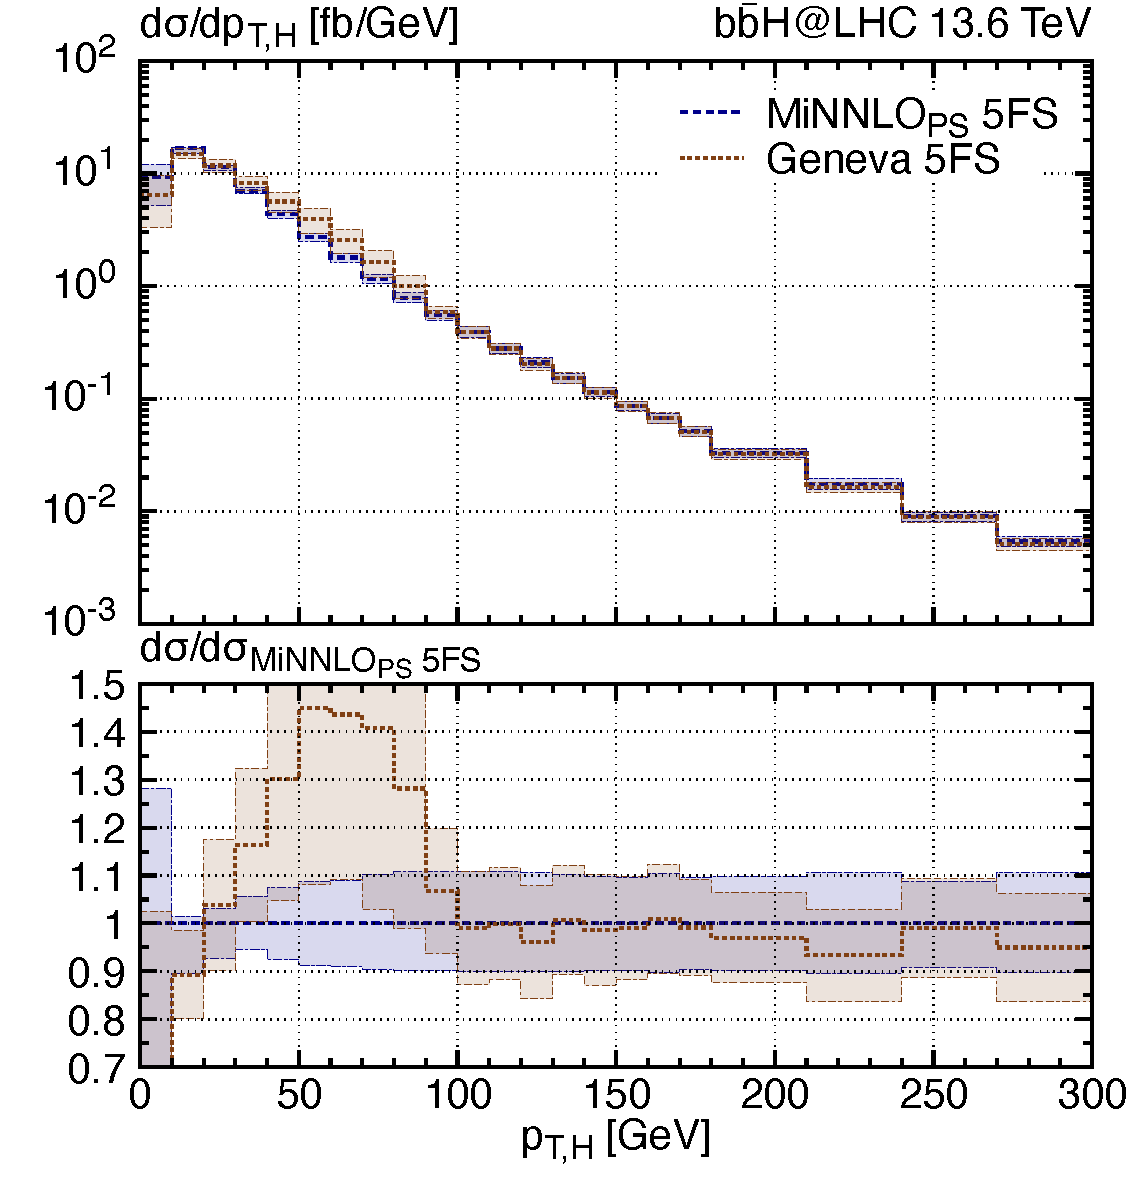
\includegraphics[width=.45\textwidth, page=1]{plots/5fs/genevaminnlo/minnloKQvar-geneva-ptH.pdf}&
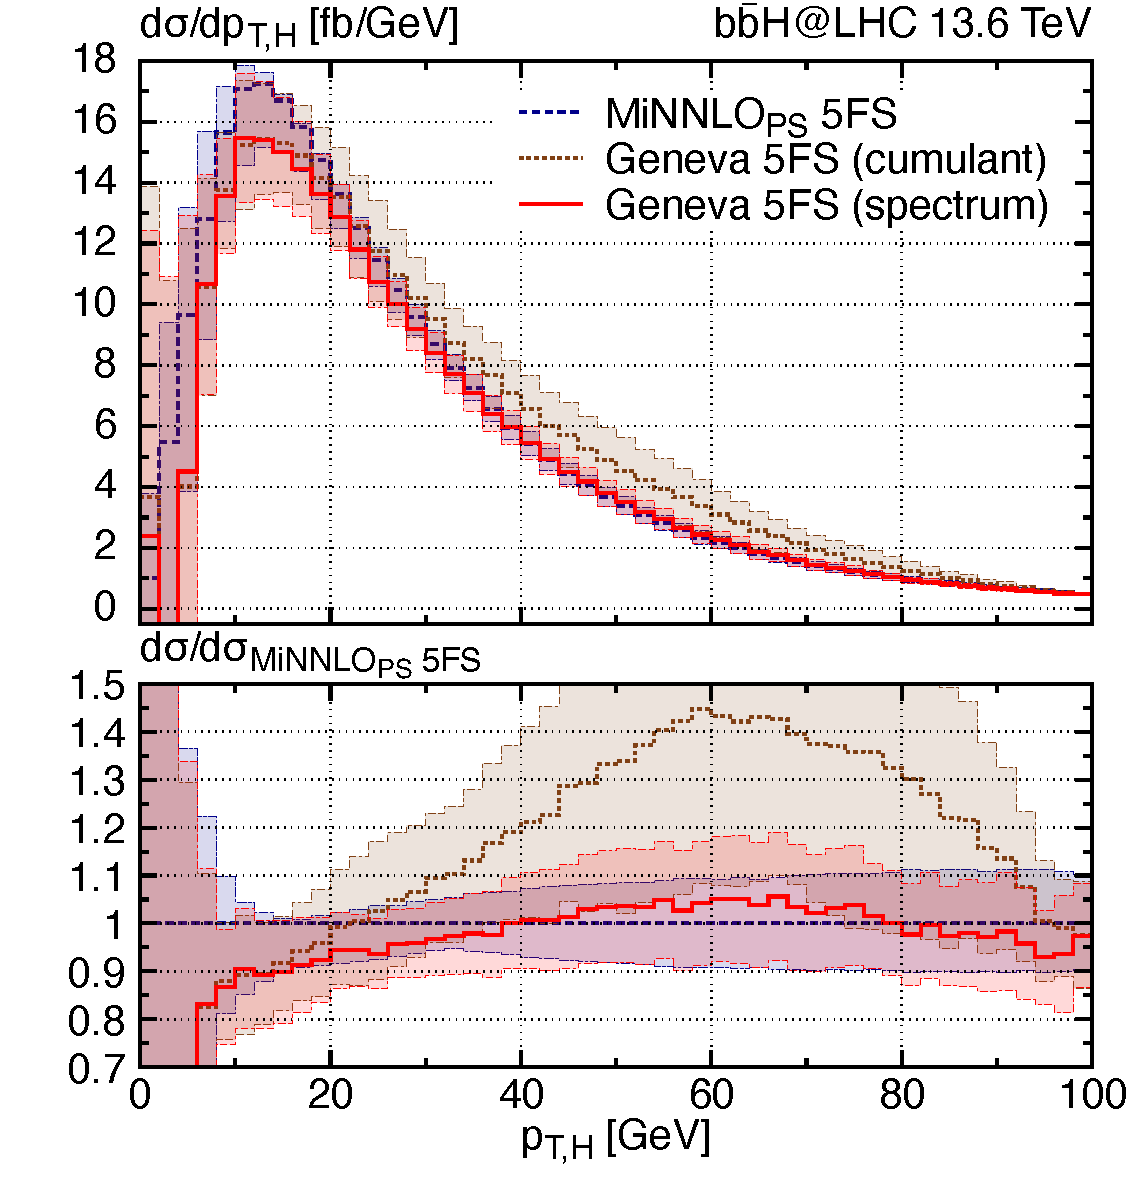
\includegraphics[width=.45\textwidth, page=1]{plots/5fs/genevaminnlo/minnloKQvar-genevaspec-ptHzoom.pdf}
\end{tabular}
\vspace*{1ex}
\caption{Comparison of \minnlo{} (blue, dashed) and \GENEVA{} (brown, dotted) predictions at NNLO+PS level for the transverse momentum distribution of the Higgs boson. The zoom version shows an alternative scale choice of the \GENEVA{} generator (red, solid).\label{fig:genevaptH}}
\end{center}
\end{figure}

\begin{figure}[t!]
\begin{center}
\begin{tabular}{cc}
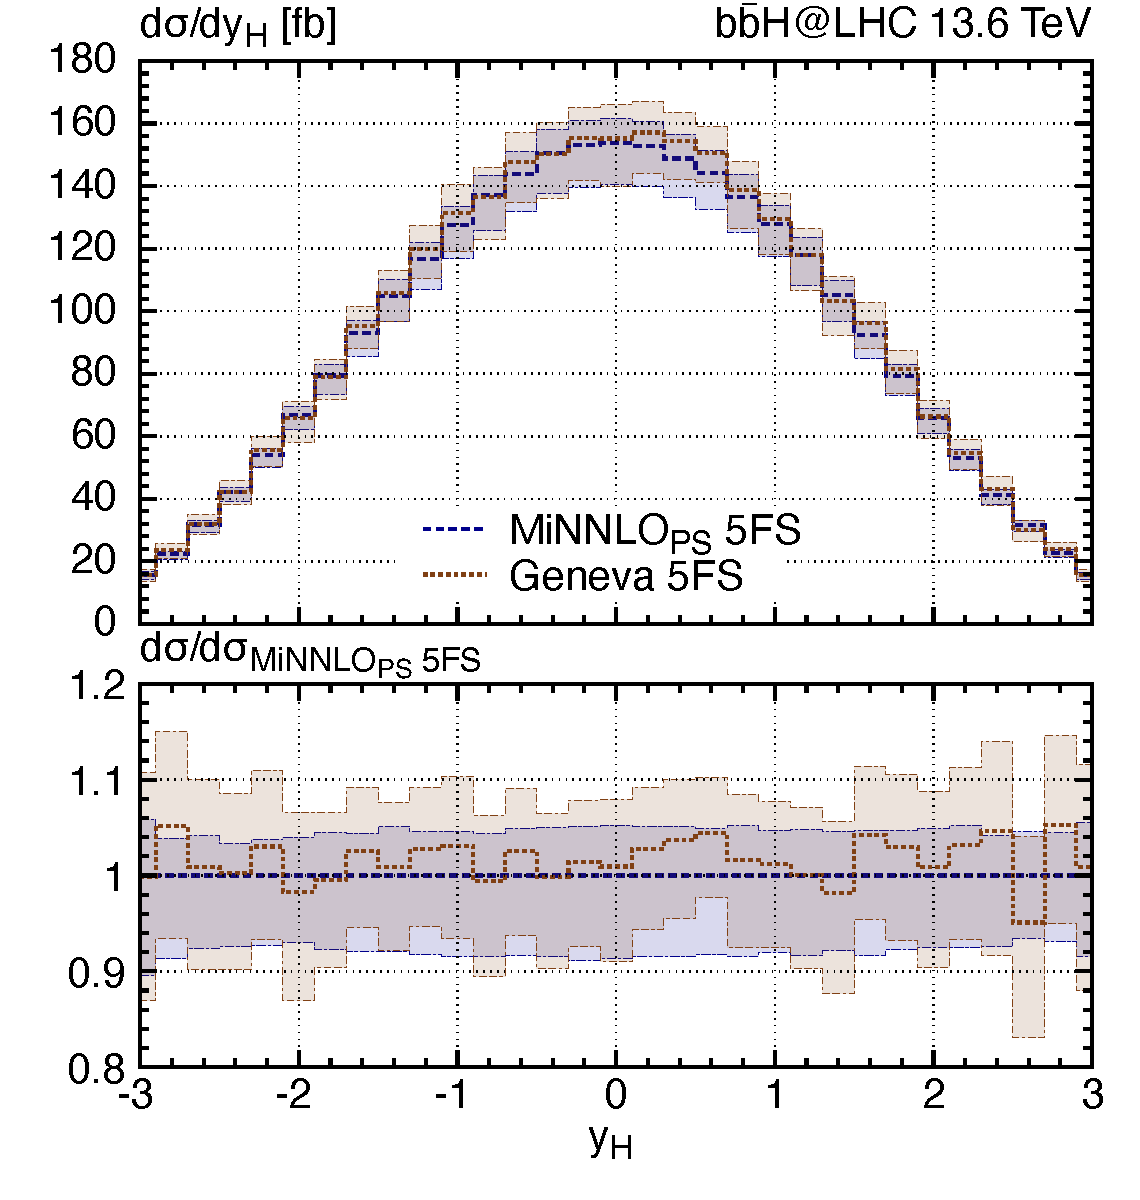
\includegraphics[width=.45\textwidth, page=1]{plots/5fs/genevaminnlo/minnloKQvar-geneva-yh.pdf}&
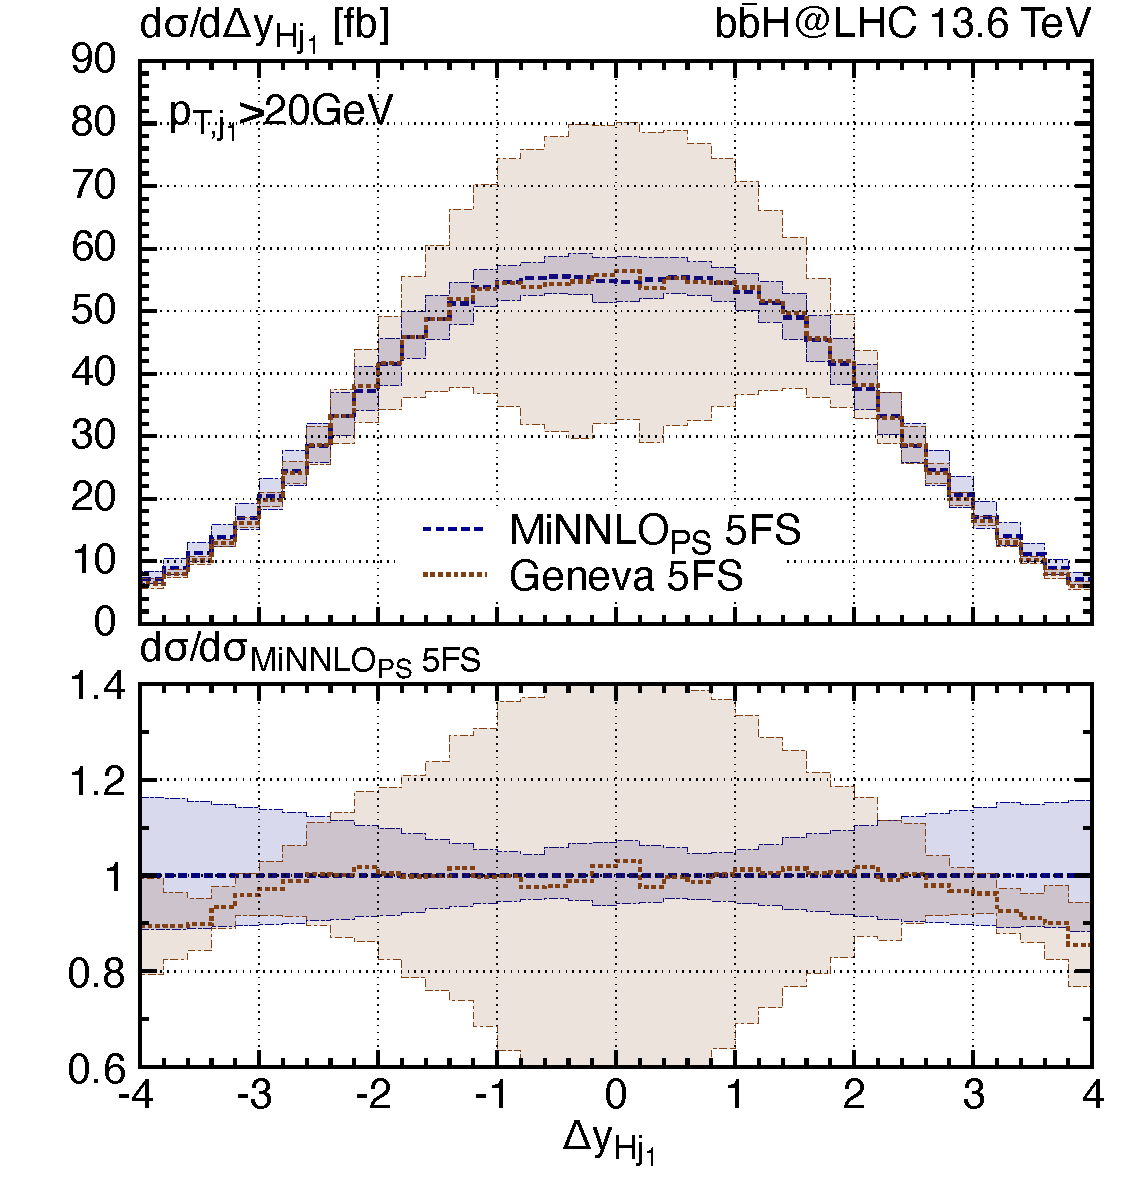
\includegraphics[width=.45\textwidth, page=1]{plots/5fs/genevaminnlo/minnloKQvar-geneva-dyhj.pdf}
\end{tabular}
\vspace*{1ex}
\caption{Higgs boson rapidity and difference in rapidity between the scalar and the leading jet as predicted by two Monte Carlo generators interfaced with \PYTHIA8{} using the \minnlo{} (blue, dashed) and \GENEVA{} (brown, dotted) methods. \label{fig:genevay}}
\end{center}
\end{figure}

\subsubsection{Transverse-momentum spectrum against resummed predictions}

\subsubsection{Heavy-Higgs for BSM studies in \minnlo{}}

The Higgs production in association with a bottom-quark pair is of particular interest in extensions beyond the Standard Model. Indeed, many BSM scenarios predict modifications to the Higgs-bottom quark coupling, which could lead to observable deviations in the production rates and kinematic distributions of the \bbH{} process. In some models, \bbH{} can become the dominant production mode of exotic Higgs states. The \minnlo{} generator presented in section~\ref{sec:5FSNNLOPS} is built within the Standard Model framework, but can be easily extended to accommodate BSM predictions. To illustrate its potential, we consider a specific example of how the NNLO+PS generator can be adapted for BSM scenarios. We specifically consider the Minimal Supersymmetric Standard Model (MSSM)~\cite{Ovrut:1984uc,Haber:1984rc,Gunion:1984yn}, which corresponds to a Type-II Two-Higgs-Doublet Model (2HDM)~\cite{Branco:2011iw} at leading order but deviates from it at higher orders. MSSM enforces relations between the Higgs sector and the superpartners of SM particles. Unlike the SM, the MSSM requires two Higgs doublets ($H_u$ and $H_d$) to give mass to both up-type and down-type fermions. An important parameter of the model is the ratio of vacuum expectation values ($v_u$ and $v_d$) of the two SU(2) doublets,
\begin{align}
	\tan\beta=\frac{v_u}{v_d}\,.
\end{align}
The other indipendent parameter is the CP-even Higgs mixing angle $\alpha$. This results in five physical Higgs bosons: two CP-even (H,H'), one CP-odd (A) and two charged Higgs bosons ($\text{H}^{\pm}$). The lightest Higgs boson ($\text{H}$) in MSSM can mimic the SM Higgs, but has different properties depending on model parameters. The tree-level mass of $\text{H}$ is bounded from above by $m_Z |\cos 2\beta|$, where $m_Z$ is the Z-boson mass. However, radiative corrections (mainly from the SUSY partners of the bottom and top quarks) can significantly alter the tree-level prediction, allowing for $m_H\sim 125$ GeV~\cite{Heinemeyer:2011aa,Bechtle:2012jw,Draper:2016pys,Bechtle:2016kui,Haber:2017erd}. We perform the NNLO+PS prediction in the benchmark configuration known as $M_H^{125}$ scenario~\cite{Bagnaschi:2018ofa}, where all superparticles are chosen to be so heavy that the presence of these effects has only a mild impact on the production and decay of MSSM Higgs bosons. As a result, the phenomenology of this scenario at the LHC closely resembles that of a Type-II 2HDM with Higgs couplings inspired by the MSSM. For the chosen mass of the supersymmetric partners, we refer to eq. (4) of~\citere{Bagnaschi:2018ofa}. SUSY particles affect the bottom Yukawa coupling, encoded on the resummation of loop-induced effects, which are $\tan\beta$-enhanced. We stress that the NNLO+PS calculation in the massless scheme contains only terms proportional to the squared bottom Yukawa coupling. As a result, predictions in the MSSM scenario differ from those in the SM solely by an overall rescaling factor. In the case of the CP-odd Higgs production, we have:
\begin{align}
	\dd \sigma_{b\bar b \text{A}}^{\text{MSSM}} = \dd \sigma_{\bbH{}}^{\text{SM}} \cdot (\tilde g_b^{\phi})^2\,,	\label{eq:BSMYuk}
\end{align}
with
\begin{align}
	\tilde{g}_b^A = \frac{\tan \beta}{1 + \Delta_b} \left( 1 - \Delta_b \frac{1}{\tan^2\beta} \right)\,.
\end{align}
The parameter \( \Delta_b \) resums higher-order sbottom contributions~\cite{Banks:1987iu,Hall:1993gn,Carena:1994bv,Carena:2000uj}. Electroweak corrections from neutralinos and charginos are incorporated into \( \Delta_b \) for this benchmark, with its numerical value determined by \texttt{FeynHiggs}~\cite{Heinemeyer:1998yj,Bahl:2018qog}. 
%The parameters \( g_f^\phi \) represent the genuine Yukawa couplings, which depend on the two angles governing the Higgs-matter interactions as defined in~\tab{tab:MSSMcoup}.\\
%\begin{table}[h]
%    \centering
%    \begin{tabular}{|c|c|c|}
%        \hline
%        \textbf{Coupling} & \textbf{MSSM value} \\
%        \hline
%        $g_u^H$ &  $\cos\alpha / \sin\beta$ \\
%        $g_d^H$ &  $-\sin\alpha / \cos\beta$ \\
%        $g_u^{H'}$ & $\sin\alpha / \sin\beta$ \\
%        $g_d^{H'}$ & $\cos\alpha / \cos\beta$ \\
%        $g_u^A$ & $\cot\beta$ \\
%        $g_d^A$ & $\tan\beta$ \\
%        \hline
%    \end{tabular}
%    \caption{Relative couplings $g_f^\phi$ with respect to the SM Yukawa coupling. The bottom Yukawa values correspond to the down-type couplings.}\label{tab:MSSMcoup}
%\end{table}
As indicated by the current constraints on \( M_H^{125} \) scenario, we consider the case of a CP-odd Higgs with a mass of 1.4 TeV and \( \tan\beta = 20 \), a point in the parameter space which is currently not excluded. In this scenario, the lightest Higgs has a mass consistent with experimental observations. We have performed the predictions by running the \minnlo{} 5FS generator with a heavy Higgs-boson mass and adjusted the Yukawa coupling according to~\eqn{eq:BSMYuk}.

\begin{figure}[t!]
\begin{center}
\begin{tabular}{cc}
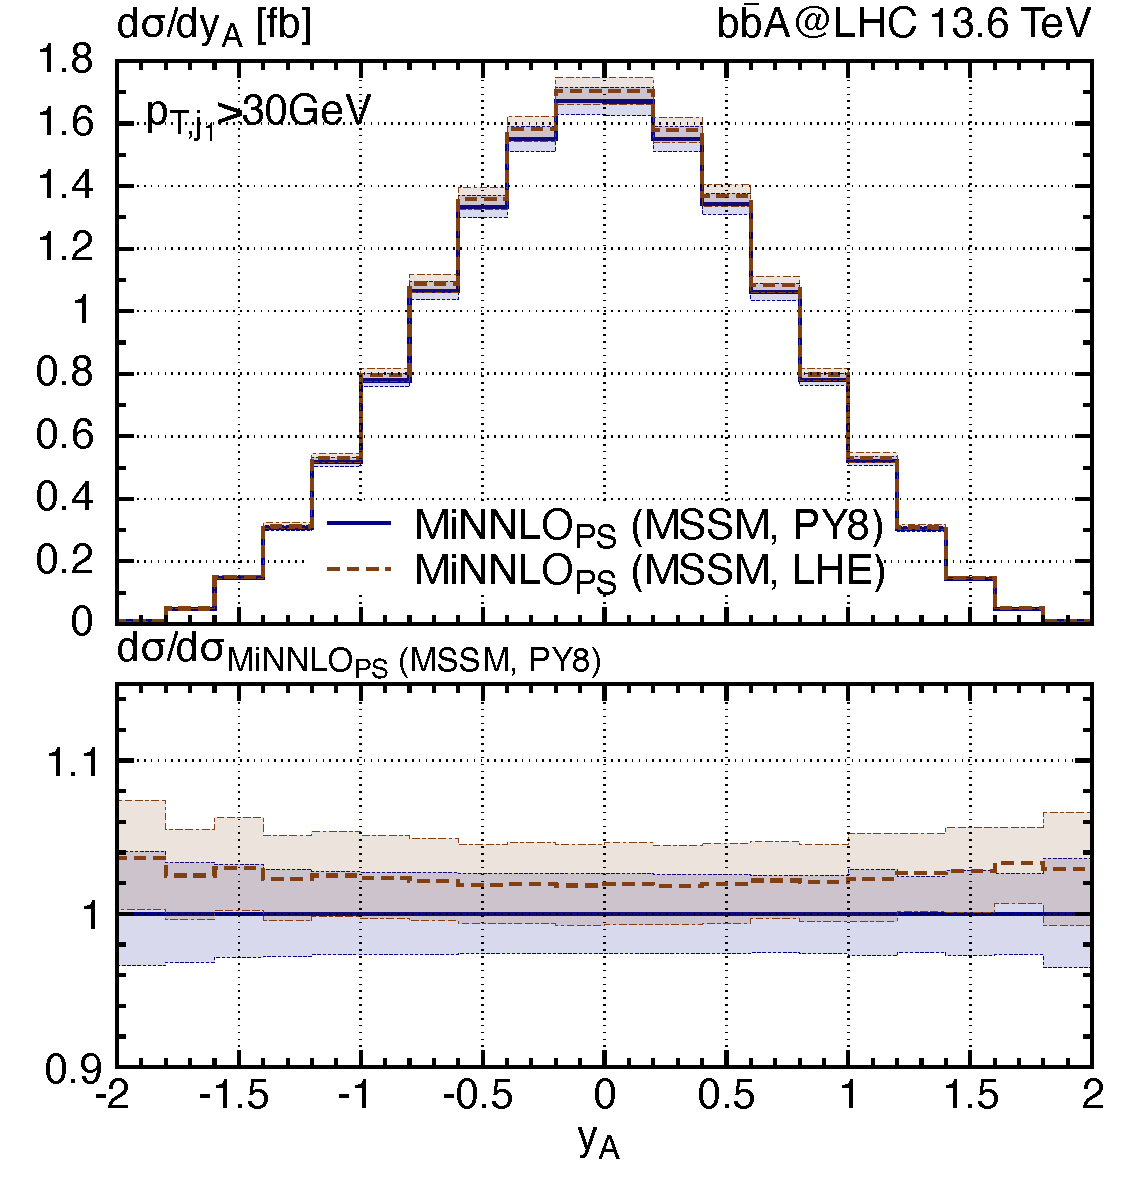
\includegraphics[width=.45\textwidth, page=1]{plots/5fs/BSM/y_H-ptj30__A-1400GeV-.pdf}&
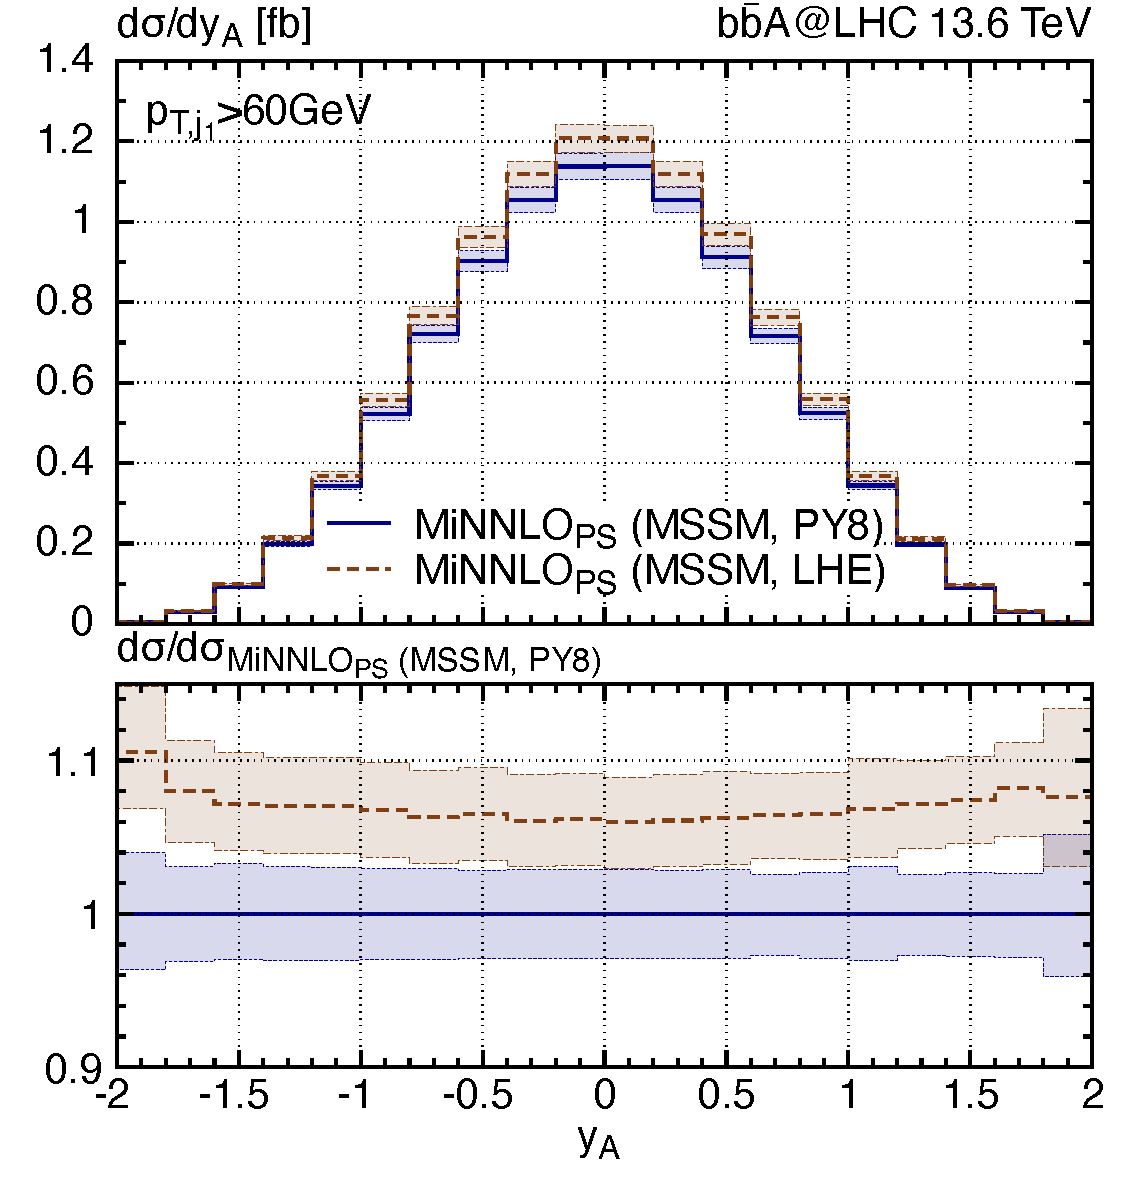
\includegraphics[width=.45\textwidth, page=1]{plots/5fs/BSM/y_H-ptj60__A-1400GeV-.pdf}
\end{tabular}
\vspace*{1ex}
\caption{Comparison of \minnlo{} results before (LHE) and after (PY8) parton shower for CP-odd Higgs rapidity spectrum. \label{fig:yA}}
\end{center}
\end{figure}

\begin{figure}[t!]
\begin{center}
\begin{tabular}{cc}
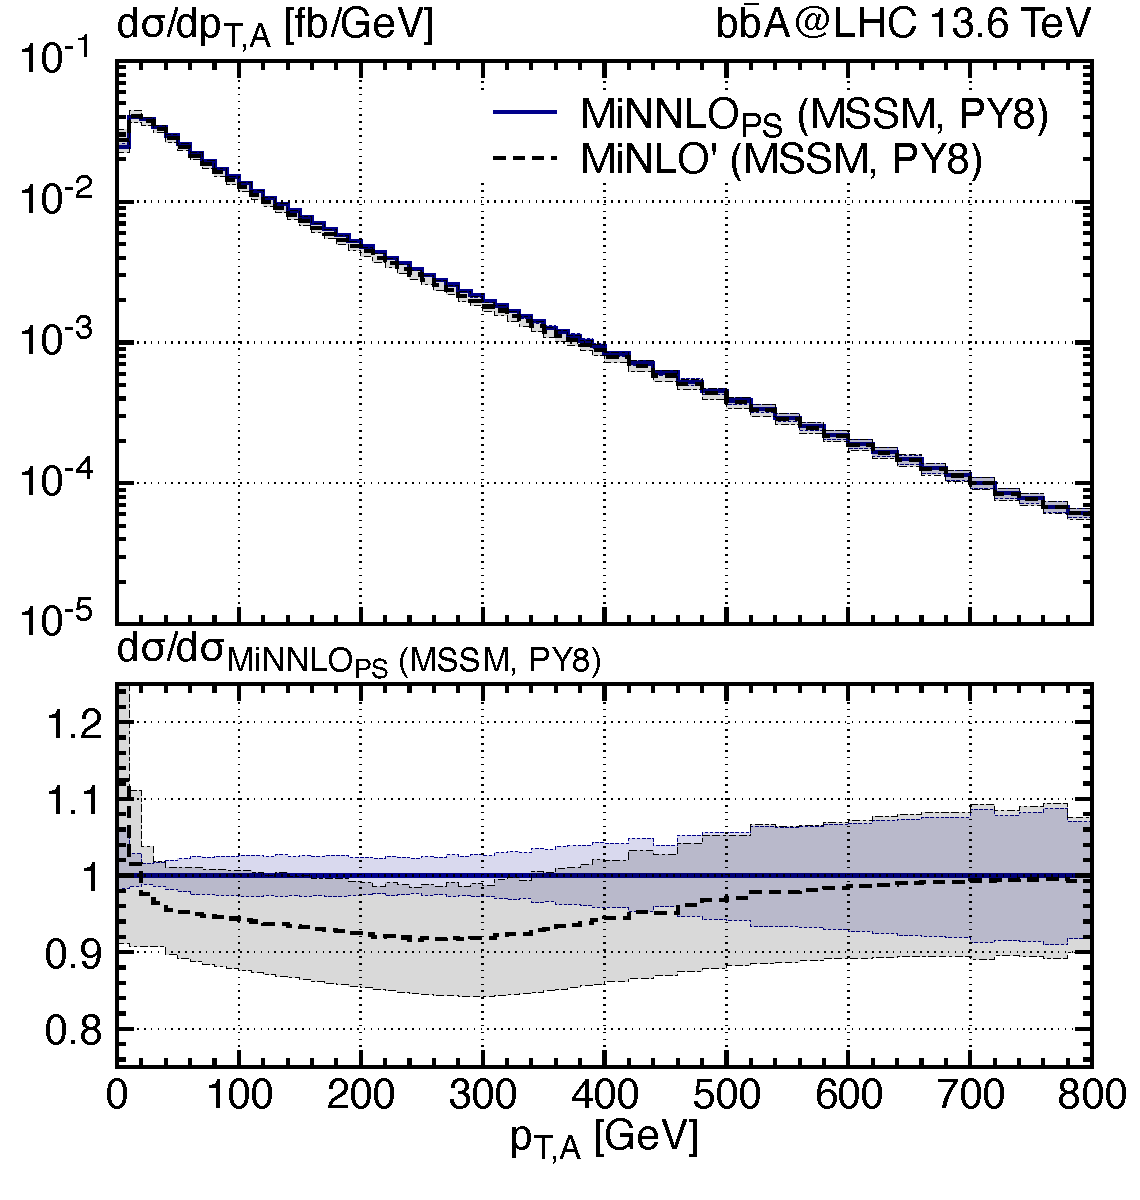
\includegraphics[width=.45\textwidth, page=1]{plots/5fs/BSM/pt_Higgs__A-1400GeV-PY8-kQ0.pdf}&
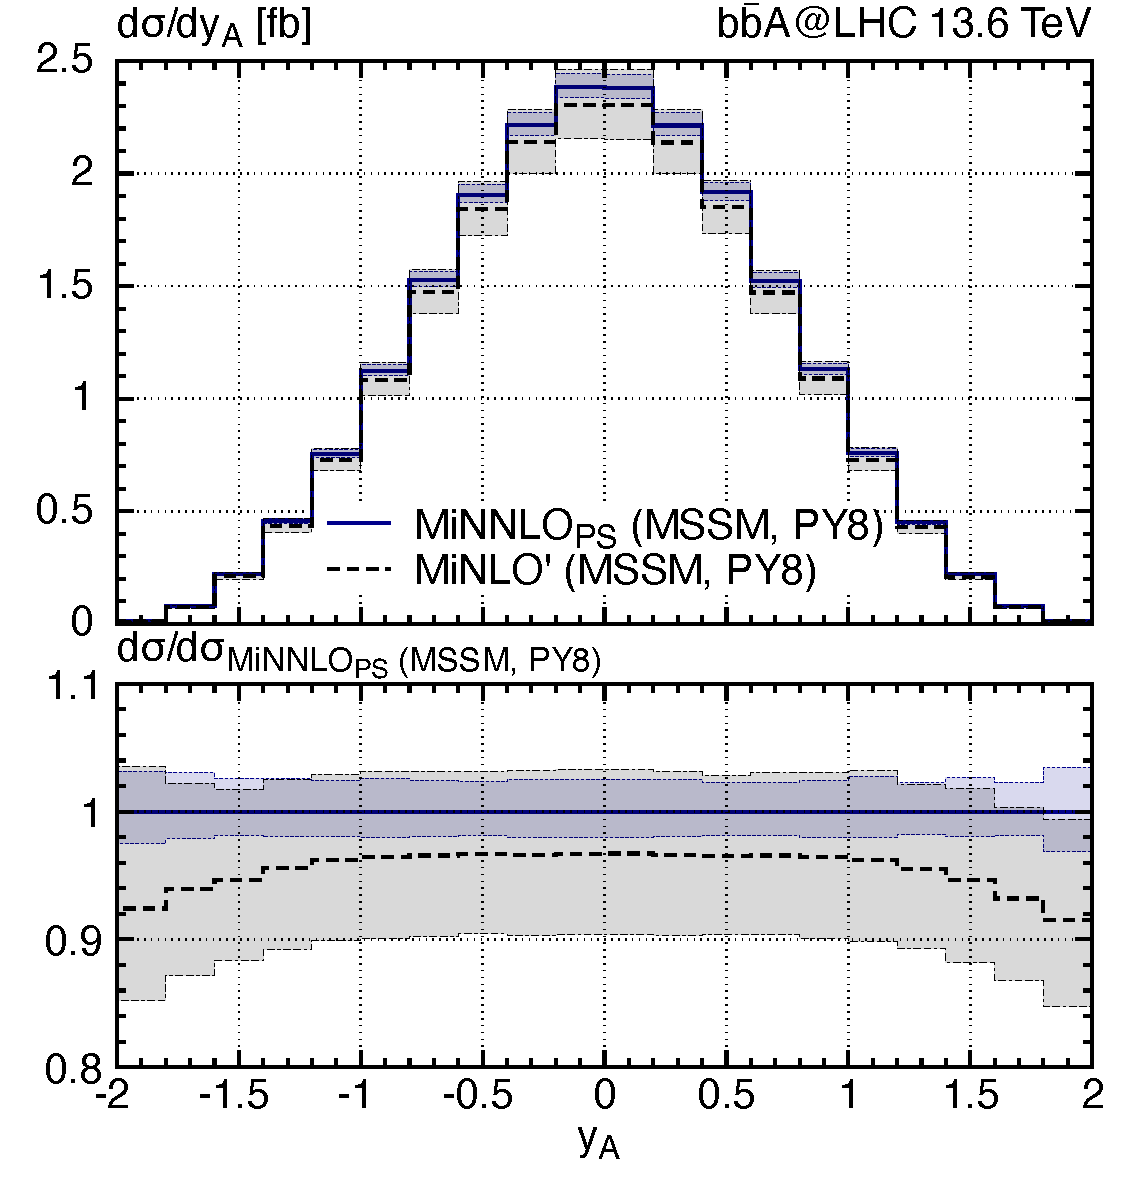
\includegraphics[width=.45\textwidth, page=1]{plots/5fs/BSM/y_Higgs__A-1400GeV-PY8-kQ0.pdf}
\end{tabular}
\vspace*{1ex}
\caption{Comparison of \minlo{} and \minnlo{} results for CP-odd Higgs rapidity spectrum with $m_A=1.4$ TeV and $\tan\beta=20$. \label{fig:MiNLOBSM}}
\end{center}
\end{figure}

\begin{figure}[t!]
\begin{center}
\begin{tabular}{cc}
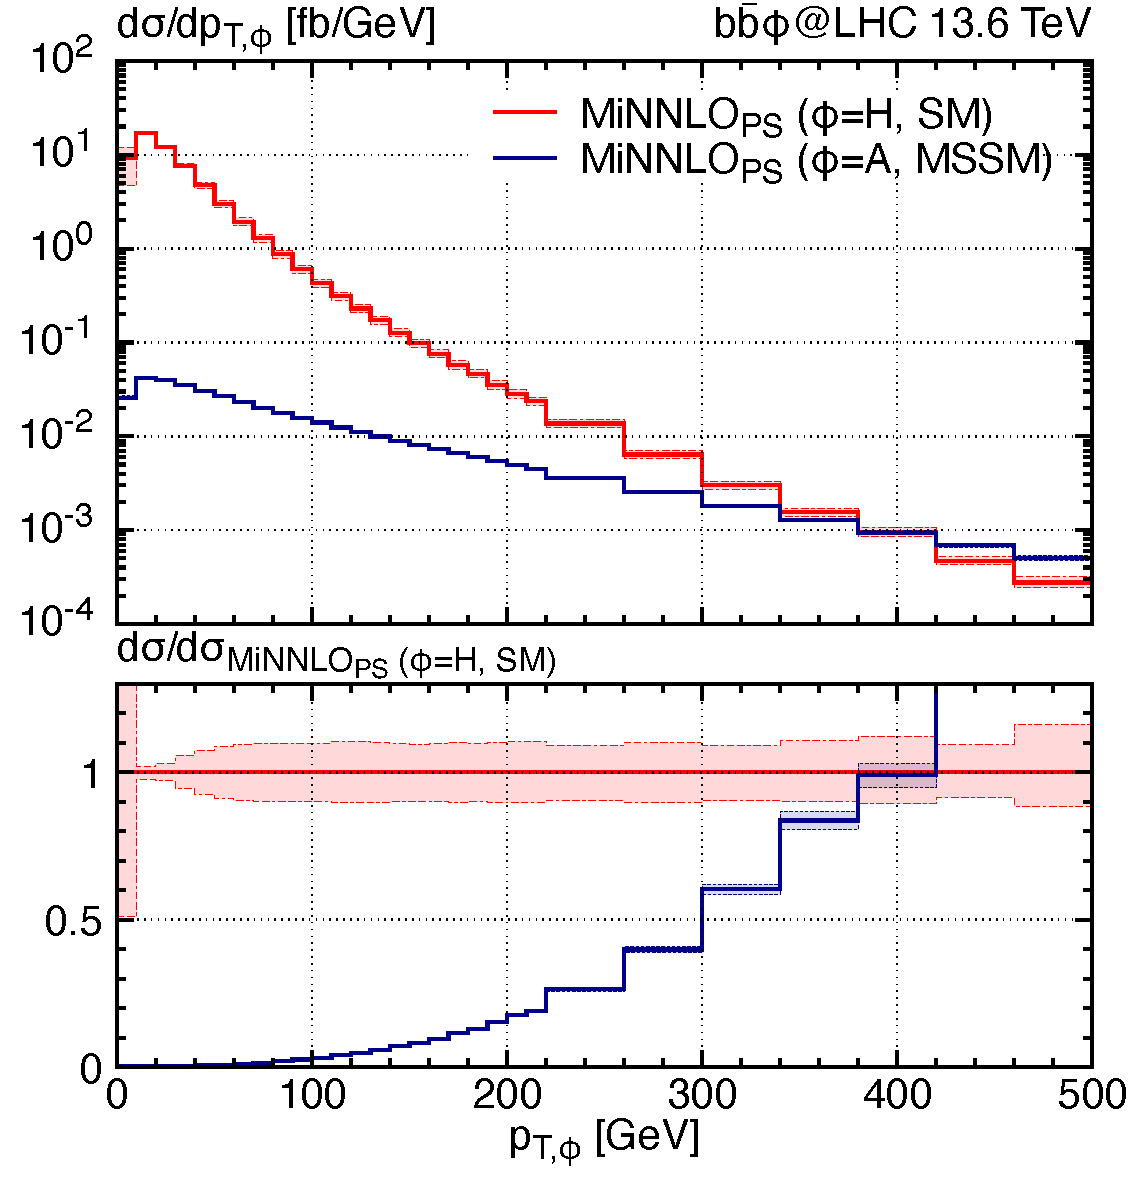
\includegraphics[width=.45\textwidth, page=1]{plots/5fs/BSM/pt_Higgs.pdf}&
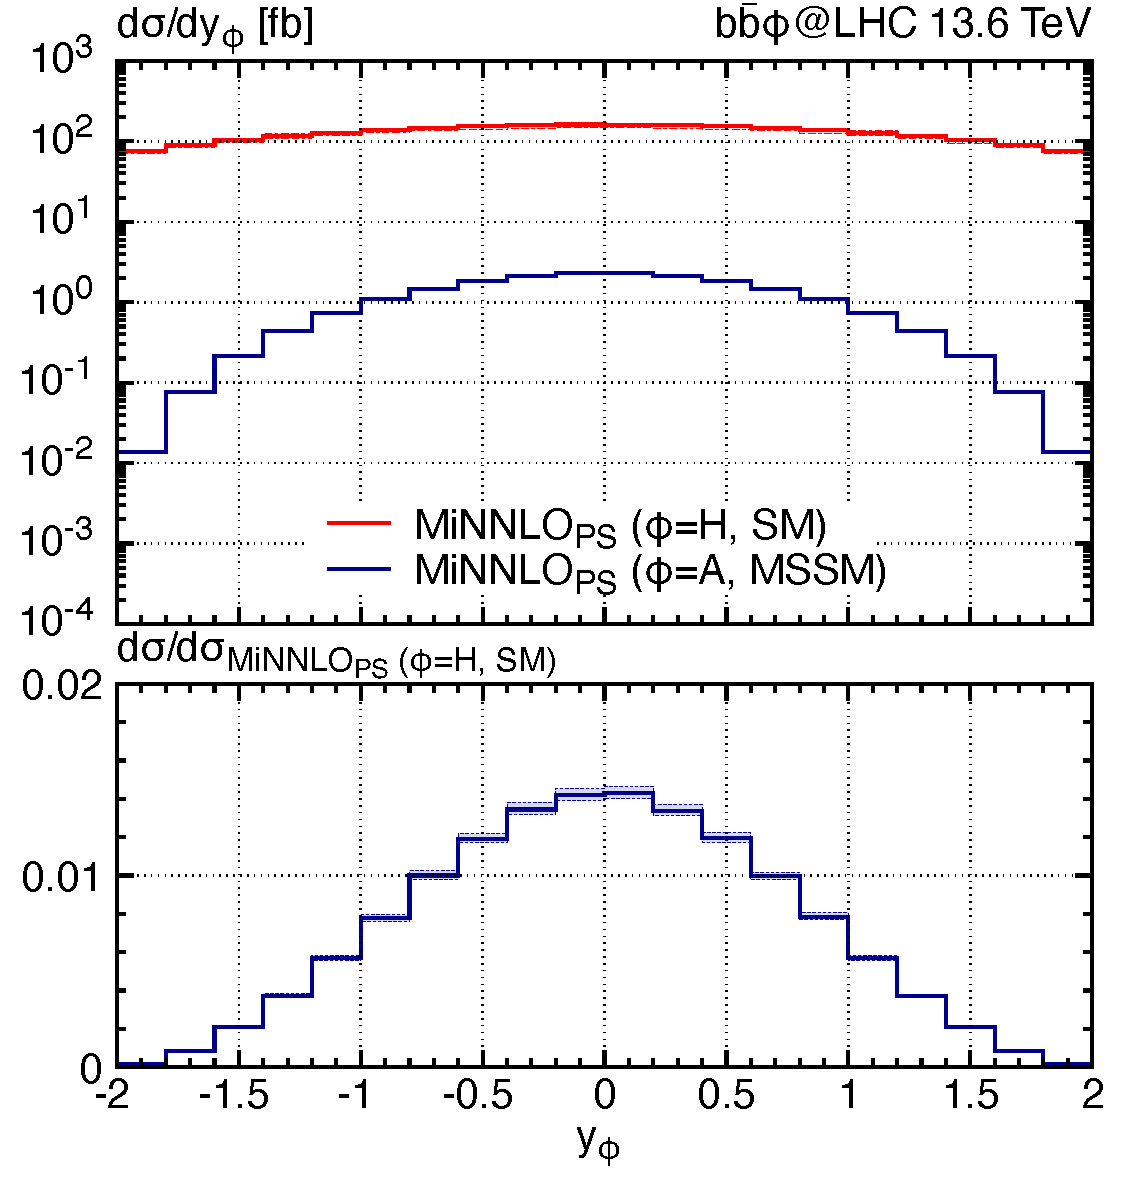
\includegraphics[width=.45\textwidth, page=1]{plots/5fs/BSM/y_Higgs.pdf}
\end{tabular}
\vspace*{1ex}
\caption{Higgs transverse momentum and rapidity spectra for \minnlo{} results with the heavy CP-odd Higgs $\text{A}$ compared to SM predictions.\label{fig:SMvsBSM}}
\end{center}
\end{figure}

In~\fig{fig:yA}, we present a comparison of the rapidity distribution of the Higgs boson A in an exclusive phase-space region. We compare the results before and after interfacing the LHE events with Pythia 8. The jet spectrum becomes slightly harder after the shower. Consequently, the NNLO+PS prediction leads to higher rapidity spectra in the presence of a transverse momentum cut of 30 GeV and 60 GeV for the leading jet. As expected, we verified that in the absence of jet cuts, the shower does not change the Higgs rapidity.  

We now turn to~\fig{fig:MiNLOBSM}, where we present a comparison between \minnlo{}  and \minlo{} predictions for the CP-odd Higgs. Due to the high mass of the bosonic state, the resummation region extends over a broader range of the transverse momentum spectrum compared to the SM Higgs, with a mass of 125 GeV. As a result, the NNLO corrections present in \minnlo{} have a greater impact even at intermediate transverse momentum values, leading to more accurate predictions and smaller scale uncertainties compared to the \minlo{} ones. In the second plot of~\fig{fig:MiNLOBSM}, we compare the two predictions for the Higgs rapidity spectrum: NNLO corrections increase the cross-section while having a flat effect in the central region $|y_A|<1$. Notably, the NNLO effects encoded in \minnlo{} are positive in the case of heavy-Higgs mass, compared to the SM case where the authors of~\citere{Biello:2024vdh} have observed a flat negative correction in the Higgs rapidity spectrum.

Finally, we compare the differential behaviour of \minnlo{} predictions for the heavy Higgs state with the SM distributions in~\fig{fig:SMvsBSM}. As expected, the BSM transverse momentum spectrum is harder. With the chosen settings, BSM effects become at least half as large as, or even larger than, the SM effects for transverse-momentum values greater than 300 GeV. In the right plot of~\fig{fig:SMvsBSM}, we compare the rapidity distributions. The heavy CP-odd Higgs exhibits a spectrum more concentrated at small rapidity values, with its contribution remaining always below 2\% of the SM prediction. We stress that the numerical comparison is highly sensitive to the choice of the MSSM parameters. However, the purpose of this analysis is not to focus on a specific choice of the MSSM parameters, but to demonstrate the potential of the \minnlo{} generator for BSM modeling of \bbH{} production at NNLO+PS.

\subsection{Bottom-Yukawa squared contribution at NNLO+PS in 4FS}
Based on \cite{Biello:2024pgo} with \minnlo{}.\cbcom{NNLO-LC reweighting ready. NNLO-FC running.} \cbcom{Explain the yukawa nf=4 with decoupling from nf=5 alphas.}
NLO+PS 5FS vs NLO+PS 4Fs and \minnlo{} 5FS vs \minnlo{} 4FS at fully-integrated level and one distribution (pt?).

\begin{table}[ht!]
  \vspace*{0.3ex}
  \begin{center}
	   \renewcommand{\arraystretch}{1.3}
    \begin{tabular}{|c||c|c|c|c|}
    \hline
      \makecell[c]{\shortstack{\rule{0pt}{2ex}Fiducial region}} &  \makecell[c]{\shortstack{\rule{0pt}{2ex}NLO+PS \\ (5FS)} } & \makecell[c]{\shortstack{\rule{0pt}{2ex}NLO+PS \\ (4FS)} }  & \makecell[c]{\shortstack{\rule{0pt}{2ex}\minnlo{} \\ (5FS)} } &  \makecell[c]{\shortstack{\rule{0pt}{2ex}\minnlo{} \\ (5FS)} } \\
     \hline \hline
	    H &  &  & & \\
     \hline
	    H $+\geq1\,bj_{\text{IFN}}$ &  &  & & \\
      \hline
	    H $+\geq2\,bj_{\text{IFN}}$ &  &  & &  \\
       \hline
            H $+0\,bj_{\text{IFN}}$  &  &  & & \\
        \hline
    \end{tabular}
  \end{center}
  \vspace{-1em}
  \caption{
	 Cross-section values of the different \POWHEG{} generators in massless and massive schemes. \label{tab:NNLO4FS_xs}}
\end{table}

\begin{figure}[t!]
\begin{center}
\begin{tabular}{cc}
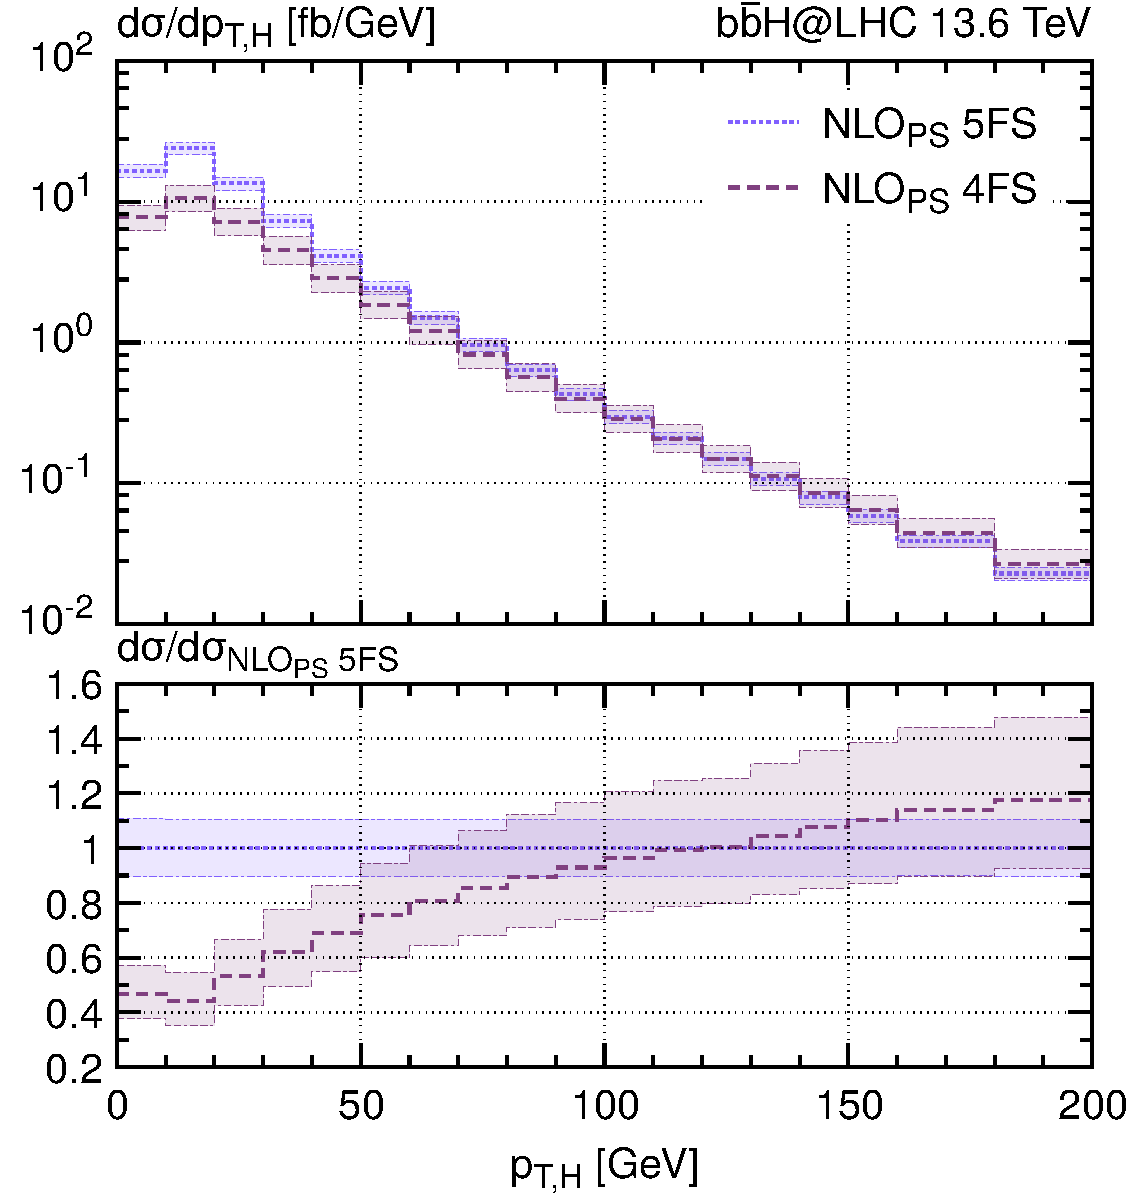
\includegraphics[width=.45\textwidth, page=1]{plots/4fs/pt_Higgs_NLO_5FS_4FS.pdf}&
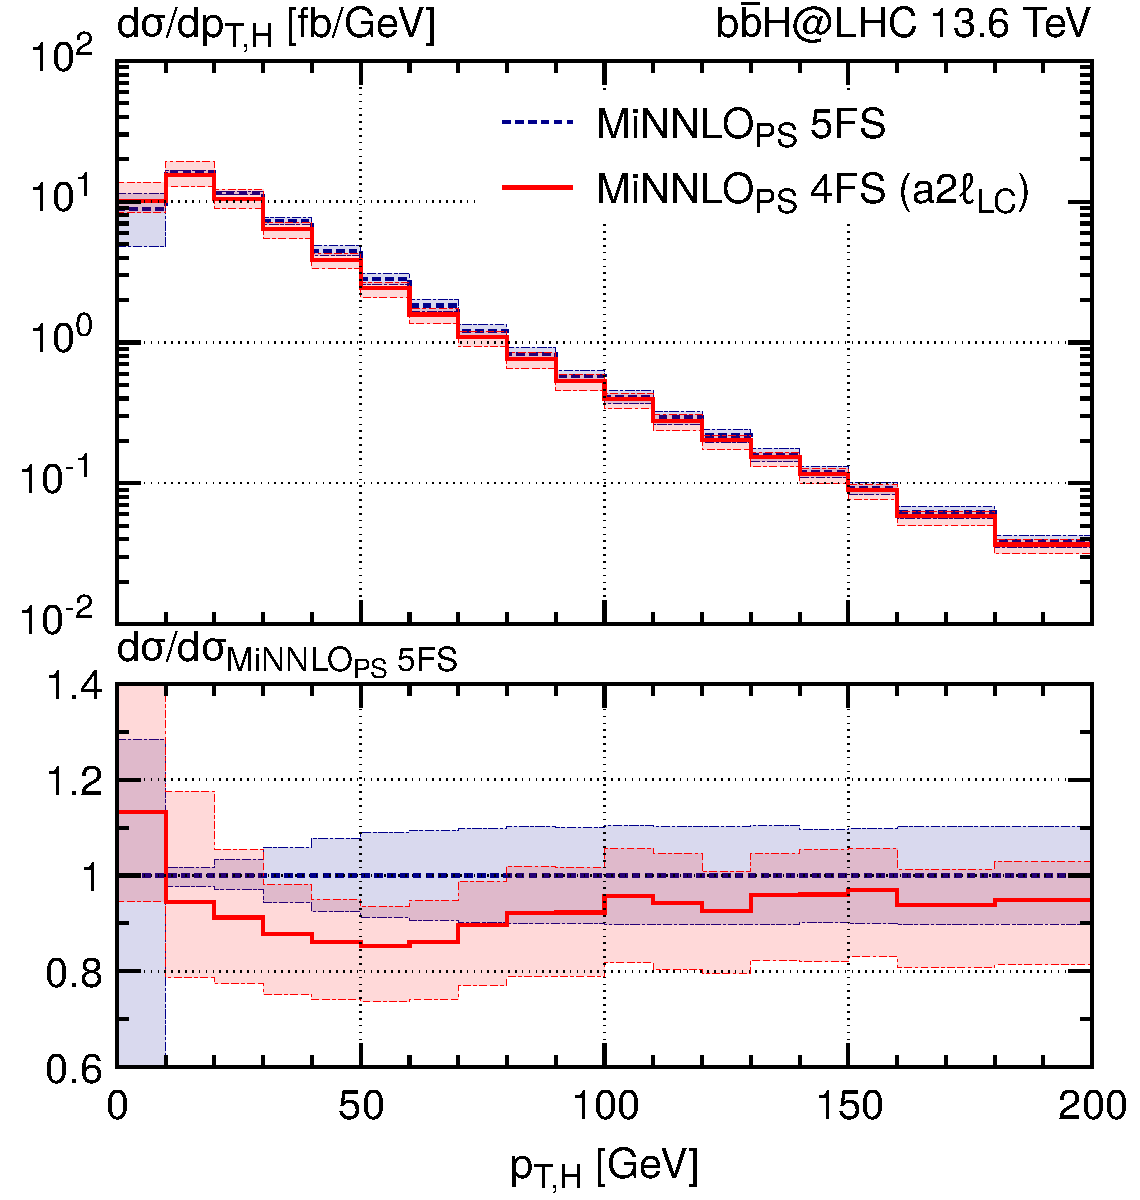
\includegraphics[width=.45\textwidth, page=1]{plots/4fs/pt_Higgs_minnlops_5FS_4FS.pdf}
\end{tabular}
\vspace*{1ex}
\caption{Comparison between different flavour scheme choices for the Higgs transverse momentum spectrum at NLO+PS (left) and NNLO+PS level (right). \label{fig:4fsA}}
\end{center}
\end{figure}

\begin{figure}[t!]
\begin{center}
\begin{tabular}{cc}
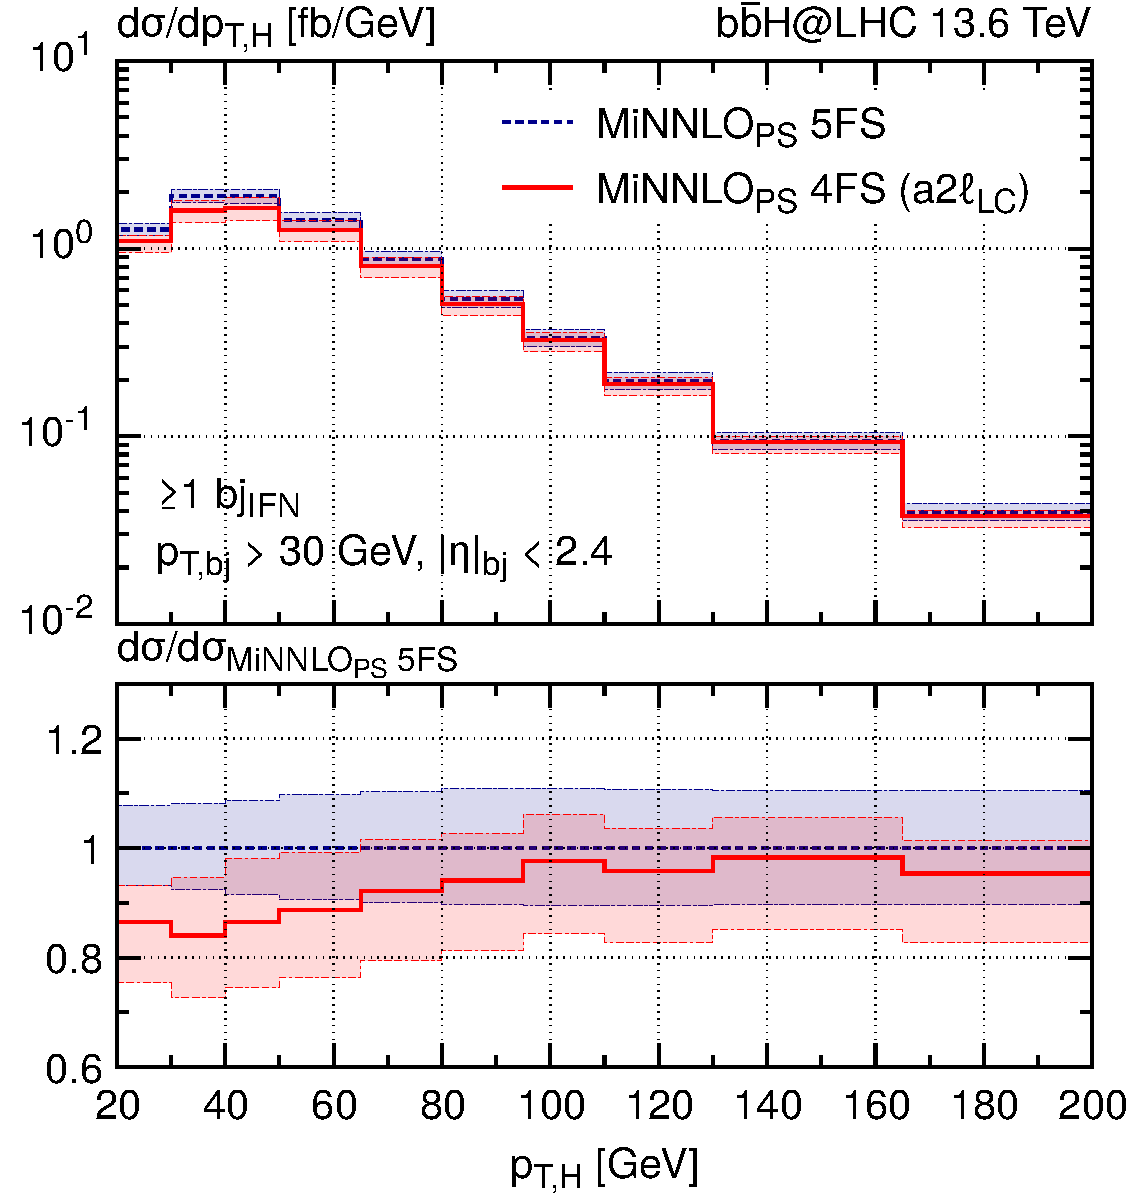
\includegraphics[width=.45\textwidth, page=1]{plots/4fs/pt_H-IFN-1bjet_minnlops.pdf}&
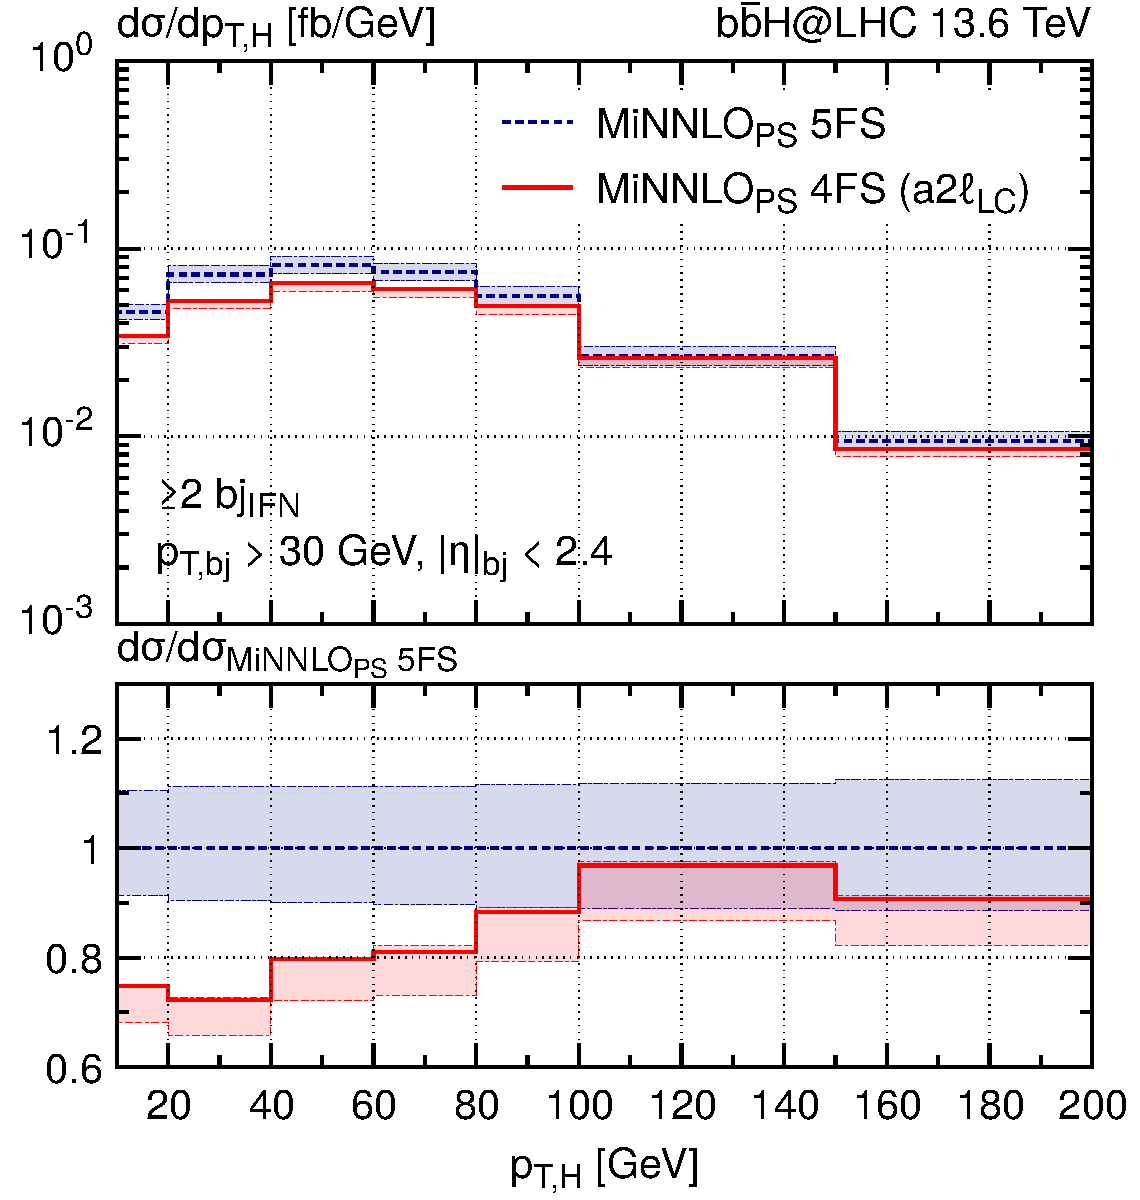
\includegraphics[width=.45\textwidth, page=1]{plots/4fs/pt_H-IFN-2bjet_minnlops.pdf}
\end{tabular}
\vspace*{1ex}
\caption{Higgs transverse momentum spectrum with at least one and two \label{fig:4fsB}}
\end{center}
\end{figure}

\section{Modelling \bbH{} for background studies in HH searches}
Focus on \citere{Manzoni:2023qaf} mainly (and \citere{Biello:2024pgo}) in fiducial cuts for HH searches (ref. Stefano Manzoni). NNLO+PS ggF generator with different $n_f$ is running using ATLAS resources.

\begin{figure}[t!]
\begin{center}
\begin{tabular}{cc}
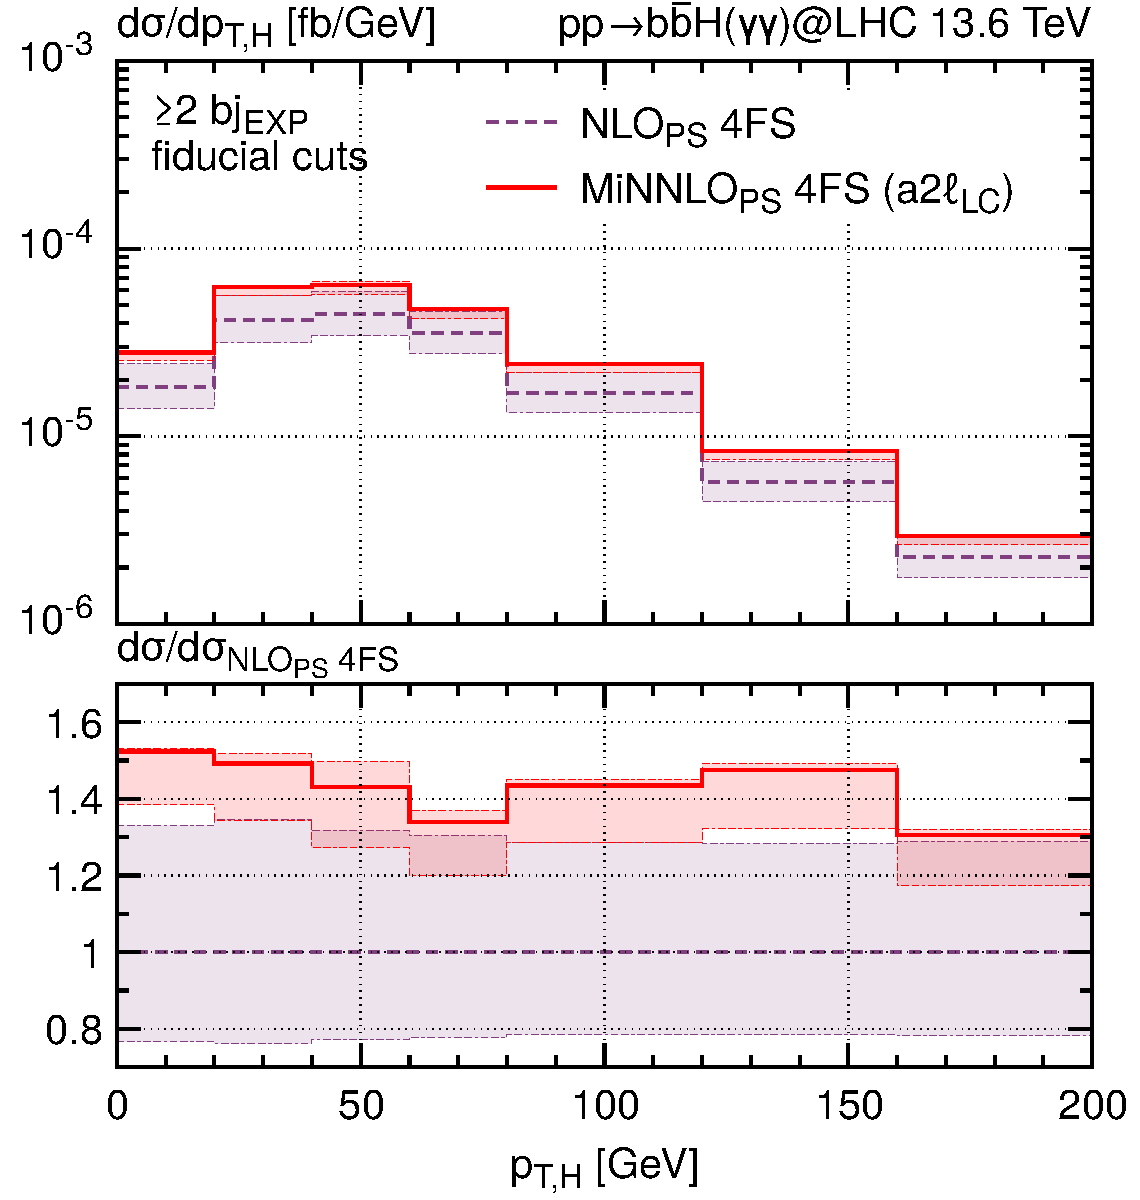
\includegraphics[width=.45\textwidth, page=1]{plots/4fs/pt_Higgs-EXP-fid.pdf}&
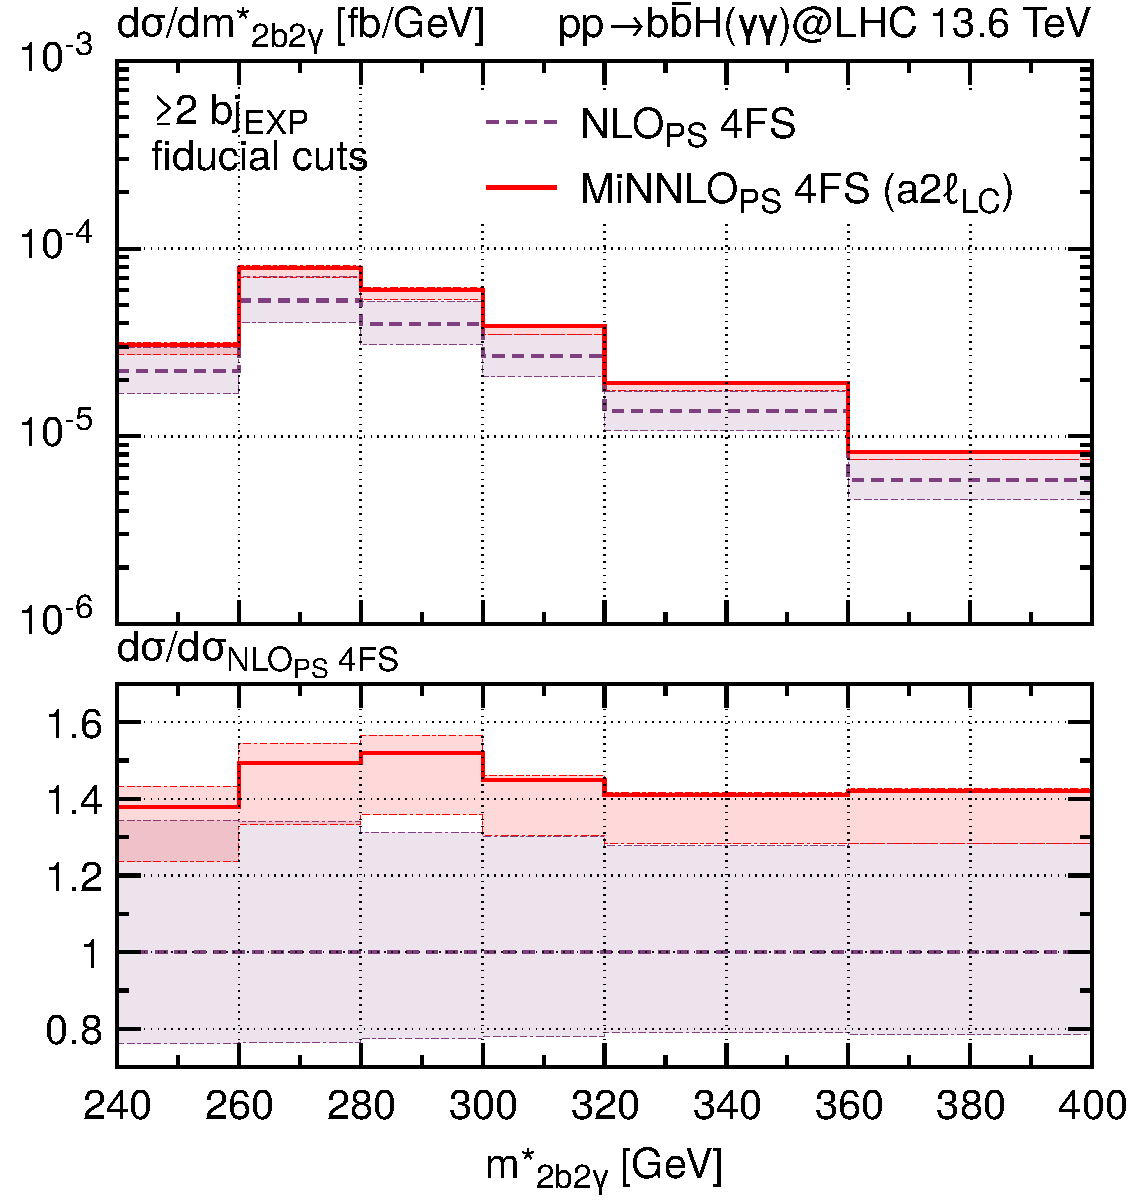
\includegraphics[width=.45\textwidth, page=1]{plots/4fs/mass_2b2gam-EXP-fid.pdf}
\end{tabular}
\vspace*{1ex}
\caption{\label{fig:4fsC}}
\end{center}
\end{figure}

\section{Light-quark Yukawa sensitivity in Higgs spectra}
\subsection{Transverse momentum resummation at N3LL'+aN3LO}
Based on \cite{Cal:2023mib} (ref. Rebecca von Kuk and Frank Tackmann).

\subsection{Novel predictions with \minnlo{}}
The \minnlo{} 5FS generator has been recently extended to light-quark parton fusion. These simulations can offer first constraints on anomalously large interactions between the Higgs boson and the light quarks. Indeed, while the bottom-quark Yukawa coupling is strongly constrained through measurements of Higgs decays, no stringent bounds exist for lighter quarks~\cite{Kagan:2014ila}. In particular, the charm Yukawa coupling is only weakly constrained, with an observed upper limit of less than 8.5 times the Standard Model prediction based on analyses of Higgs decay products in Higgsstrahlung events~\cite{Atlas:2022ers}. The development of an NNLO+PS generator for \( q\bar{q} \rightarrow H \) production can provide valuable input for setting constraints on light-quark Yukawa couplings. In particular, it enables the determination of upper bounds for the couplings of up-, down-, and strange-type quarks, owing to the cross-section enhancement driven by their parton distribution functions. 
The cross-section for single Higgs production via parton fusion is given by:
\begin{align}
	\sigma_{\text{H}}(\bar \kappa_q^2)=\sigma_{b\bar b \rightarrow \text{H}}+\bar \kappa_c^2 \bar \sigma_{c\bar c \rightarrow \text{H}}+\bar \kappa_s^2 \bar \sigma_{s\bar s \rightarrow \text{H}}+\bar \kappa_d^2 \bar \sigma_{d\bar d \rightarrow \text{H}}+\bar \kappa_u^2 \bar \sigma_{u\bar u \rightarrow \text{H}}\,.
\end{align}
All interference effects at higher orders vanish due to the massless treatment of the \( n_f = 5 \) parton species. In this context, we introduce the coupling \( \bar\kappa_q \), which denotes the Yukawa coupling of a light quark \( q \), normalised to the Standard-Model Yukawa coupling of the bottom quark in the \MSbar{} scheme. As a consequence, the cross-section values \( \bar\sigma_{q\bar q \rightarrow \text{H}} \) inherit a dependence on the bottom-quark Yukawa coupling. In other words, they represent the cross sections obtained by using \( q \)-flavored PDFs and assigning the Yukawa interaction the strength of the bottom-quark coupling.

A value of \( \bar\kappa_q = 1 \) corresponds to a Yukawa coupling for quark \( q \) equal in strength to that of the bottom quark. While the SM expectation is \( \kappa_q = 1 \), the normalised couplings take the following values in the SM:  
\( \bar \kappa_u \simeq 5.17 \cdot 10^{-4} \),  
\( \bar \kappa_d \simeq 1.12 \cdot 10^{-3} \),  
\( \bar \kappa_s \simeq 2.2 \cdot 10^{-2} \).
The High-Luminosity Large Hadron Collider prospects~\cite{deBlas:2019rxi} shows that the light-quark Yukawa coupling can be constrained to $|\bar \kappa_u|\leq 0.66$, $|\bar \kappa_d|\leq 0.70$, $|\bar \kappa_s|\leq 0.66$ at 95\% CL when using the transverse momentum distribution.

The simulations are produced using the \minnlo{} \bbH{} generator in the massless scheme as a starting point. The code modifies the flavour of the initial-state partons via the \texttt{whichlightquark} flag, which is set to the Monte Carlo ID number corresponding to the chosen flavour. The generator consistently calls the appropriate analytic amplitudes, with the sole exception of the double real corrections, which are evaluated numerically using the \OpenLoops{} \texttt{bbhjj} library with a suitable flipping of the parton flavours. The number of active massless species is always set to \( n_f = 5 \), including in the running of the strong coupling and Yukawa factors. 

The theoretical uncertainty is estimated through the standard 7-point scale variation of the factorisation scale for the PDFs and the renormalisation scale with a correlated variation of Yuakwa and strong coupling scales. The events with on-shell Higgs bosons are passed to \PYTHIA{8}, where the decay into two photons is simulated using the narrow-width approximation, assuming a branching fraction of \({\rm BR}(H \to \gamma\gamma) = 0.227\%\)~\cite{LHCHiggsCrossSectionWorkingGroup:2016ypw}. Inspired by a fiducial region accessible by both the ATLAS and CMS detectors we apply the following constraints on the rapidities and transverse momenta of the two photons:
\begin{equation}
|y(\gamma_i)|< 2.37, \quad
\frac{p_T(\gamma_1)}{m(\gamma_1, \gamma_2)} > 0.35,\quad \frac{p_T(\gamma_2)}{m(\gamma_1, \gamma_2)} > 0.25\,. \label{eq:aafidmycuts}
\end{equation}
Here, \( \gamma_1 \) denotes the hardest photon, i.e., the one with the largest transverse momentum. We apply the diphoton \texttt{fiducial cuts} defined in~\eqn{eq:aafidmycuts} and reconstruct the Higgs boson momentum through the components of the photon pair.

To enable cross-checks and comparisons with fixed-order predictions, we have extended the public code \SuSHi{}~\cite{Harlander:2012pb,Harlander:2003ai} to support calculations in light-quark parton fusion. In~\tab{tab:qqH_xs} we present the fully-integrated cross-section values for the total rate of Higgs boson production predicted by the extensions of \SuSHi{} and \minnlo{} according to the setup in~\sct{sec:setup}. We stress that the values are obtained using the bottom-quark Yukawa coupling and must therefore be rescaled by the ratio of the squared quark masses to obtain the correct magnitude of the Standard Model prediction. The central values show an enhancement of the cross section at fixed Yukawa coupling, driven by the parton luminosities. We observe good agreement between the fixed-order and \minnlo{} cross-section predictions, particularly in the down- and up-quark channels. Moreover, the scale uncertainties are significantly reduced in the down, up, and strange channels compared to those involving heavier flavours, most notably the bottom-quark fusion. In the last column of~\tab{tab:qqH_xs} we report the integrated cross-section numbers from the NNLO+PS simulation over the fiducial region defined by the diphoton cuts defined in~\eqn{eq:aafidmycuts}. We stress the different order of magnitude compared to the cross-sections for on-shell Higgs production, due to the Higgs branching ratio into photons. Among the initial-state quarks, the up quark shows the lowest efficiency in passing the fiducial selection, with only about 36\% of diphoton decay events surviving the cuts, compared to approximately 44\% for the down quark and 59\% for the charm quark.
\begin{table}[ht!]
  \vspace*{0.3ex}
  \begin{center}
	   \renewcommand{\arraystretch}{1.3}
    \begin{tabular}{|c||c|c||c|}
    \hline
    \makecell[c]{Flavour channel} & \makecell[c]{\shortstack{$\bar \sigma_{q\bar q \rightarrow \text{H}}$ (pb)\\ \SuSHi{}} } & \makecell[c]{\shortstack{$\bar \sigma_{q\bar q \rightarrow \text{H}}$ (pb)\\ \minnlo{}} }&  \makecell[c]{\shortstack{$\bar \sigma_{q\bar q \rightarrow \text{H}(\rightarrow\gamma \gamma)}$ (fb)\\ \texttt{fiducial $\gamma\gamma$ cuts}\\ \minnlo{}}}  \\
     \hline \hline
	    $d \bar d \rightarrow$ H & $11.46(6)_{-1.1\%}^{+0.5\%}$ & $11.44(2)_{-2.4\%}^{+2.8\%}$ & $11.40(9)_{-2.4\%}^{+2.8\%}$ \\
     \hline
	    $u \bar u \rightarrow$ H & $16.46(6)_{-1.1\%}^{+0.6\%}$ & $16.47(1)_{-1.0\%}^{+2.7\%}$  &  $13.26(4)_{-0.7\%}^{+2.1\%}$ \\
      \hline
	    $s \bar s \rightarrow$ H & $4.45(4)_{-1.4\%}^{+1.0\%}$ & $4.47(3)_{-1.8\%}^{+4.0\%}$  & $6.21(4)_{-1.9\%}^{+4.1\%}$  \\
       \hline
       $c \bar c \rightarrow$ H & $1.84(9)_{-2.9\%}^{+1.5\%}$ & $1.77(8)_{-0.9\%}^{+2.3\%}$  &  $2.40(0)_{-1.0\%}^{+2.3\%}$ \\
        \hline
        $b \bar b \rightarrow$ H &  $0.585(0)_{-9.2\%}^{+7.0\%}$ &  $0.575(7)_{-8.0\%}^{+4.5\%}$ & $0.807(0)_{-8.2\%}^{+4.7\%}$ \\
        \hline
    \end{tabular}
  \end{center}
  \vspace{-1em}
  \caption{
	 Comparison of \SuSHi{} cross-section numbers against the integrated \minnlo{} results for Higgs boson production via light-quark annihilation, with the Yukawa couplings set to the bottom-quark value. The last column presents the NNLO+PS results for $H\rightarrow \gamma\gamma$ production within the fiducial region defined in~\eqn{eq:aafidmycuts}. \label{tab:qqH_xs}}
\end{table}

\begin{figure}[t!]
\begin{center}
\begin{tabular}{cc}
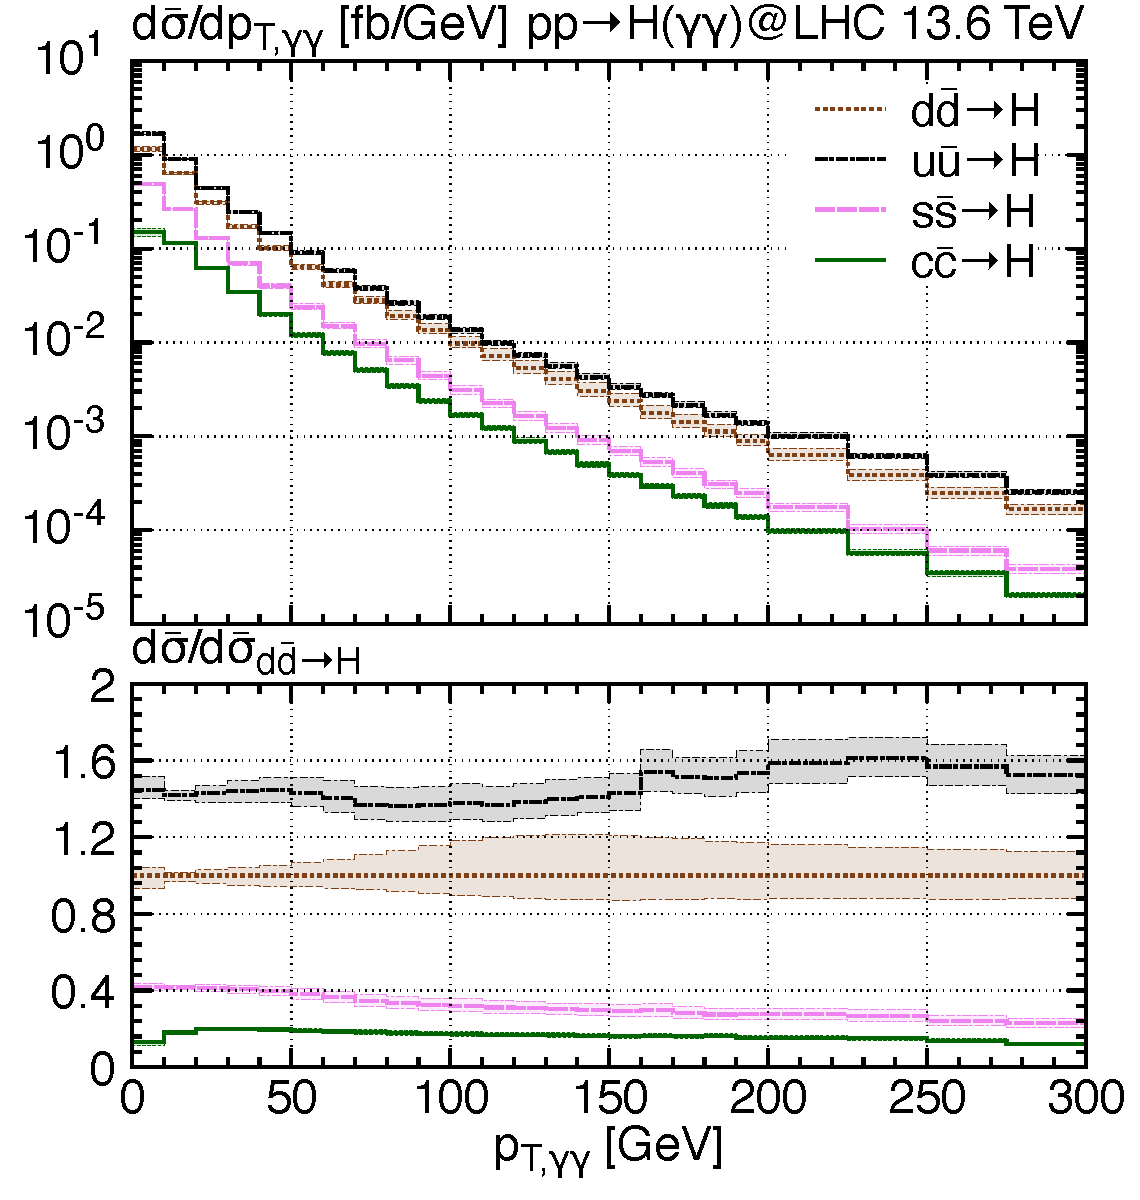
\includegraphics[width=.45\textwidth, page=1]{plots/5fs/light/ptH.pdf}&
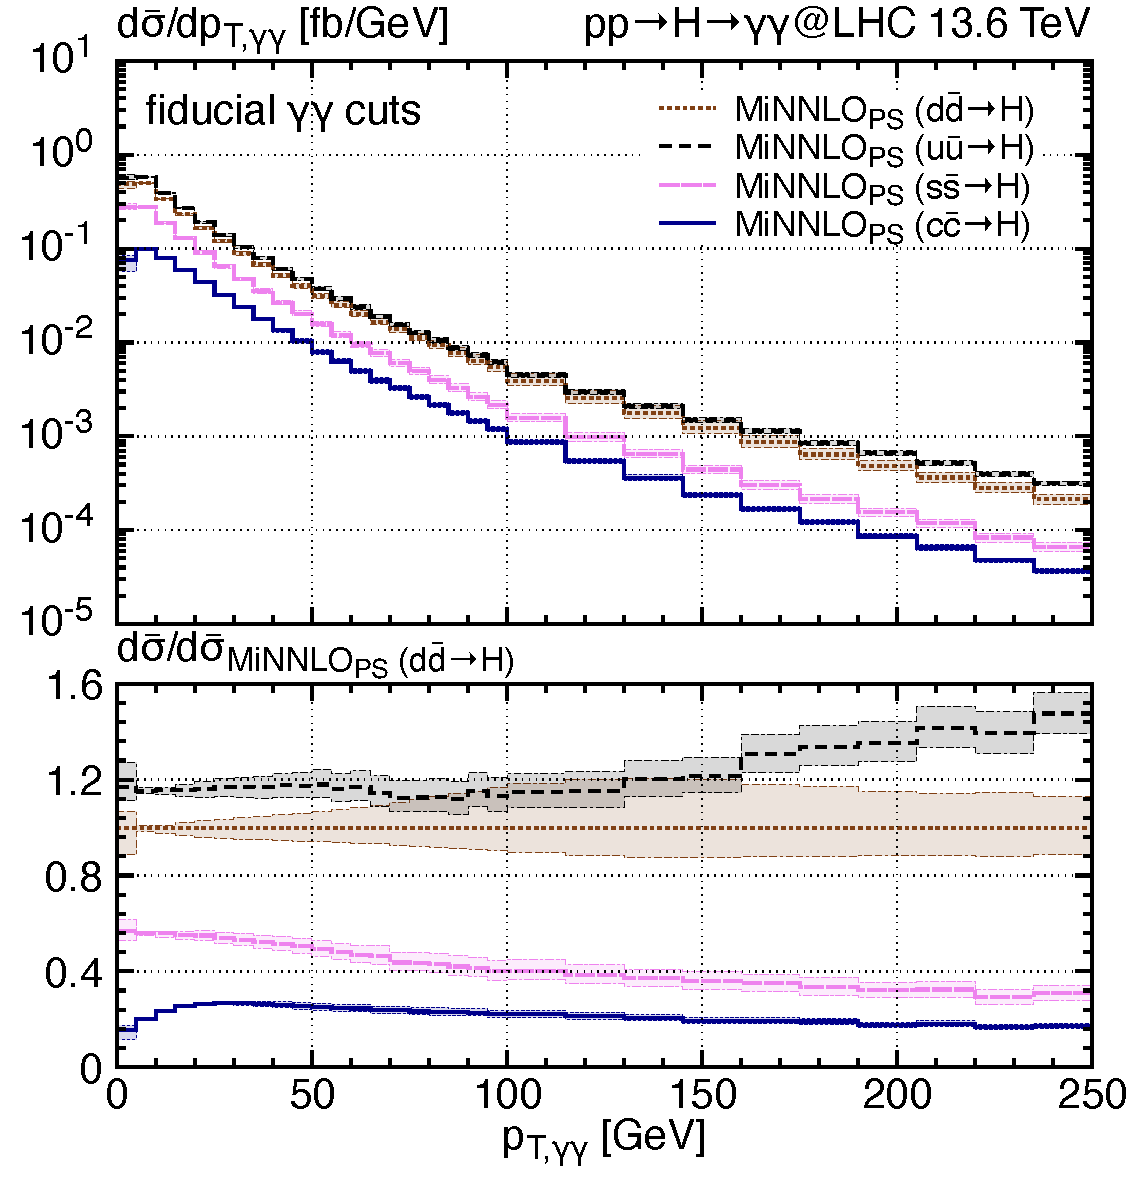
\includegraphics[width=.45\textwidth, page=1]{plots/5fs/light/pt_Higgs-aafid.pdf}
\end{tabular}
\vspace*{1ex}
\caption{Transverse momentum distribution of the reconstructed Higgs boson without cuts (left) and within the fiducial region defined in~\eqn{eq:aafidmycuts} (right).
The results are normalised to the prediction for down-quark fusion (brown, dotted) and compared to those for up- (black, short-dashed), strange- (pink, long-dashed), and charm-quark (blue, solid) fusion.
\label{fig:lightpTH}}
\end{center}
\end{figure}

\begin{figure}[t!]
\begin{center}
\begin{tabular}{cc}
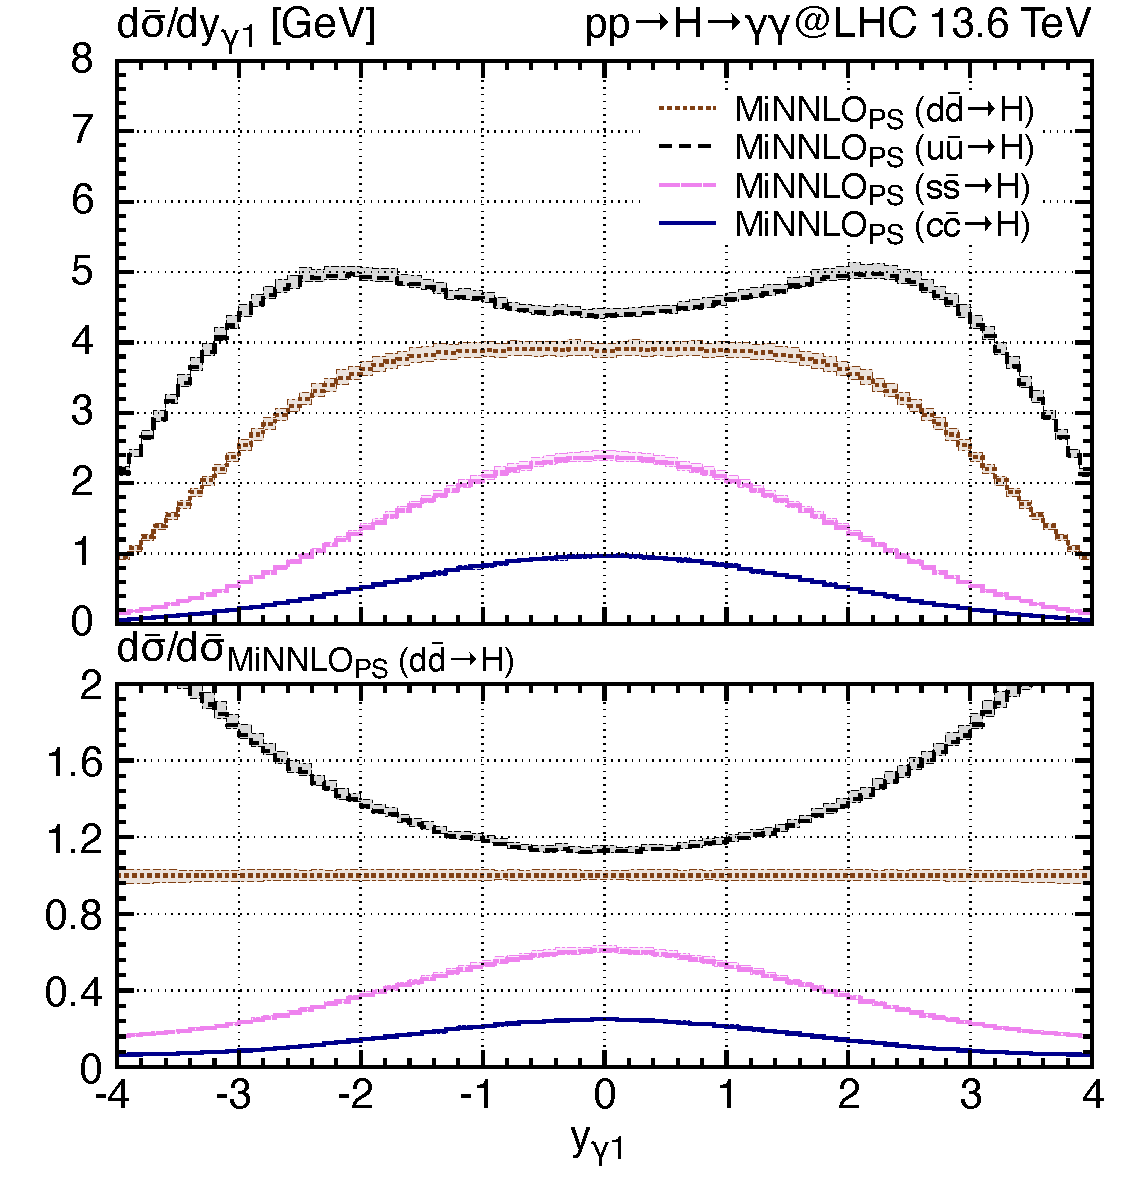
\includegraphics[width=.45\textwidth, page=1]{plots/5fs/light/yphoton1.pdf}&
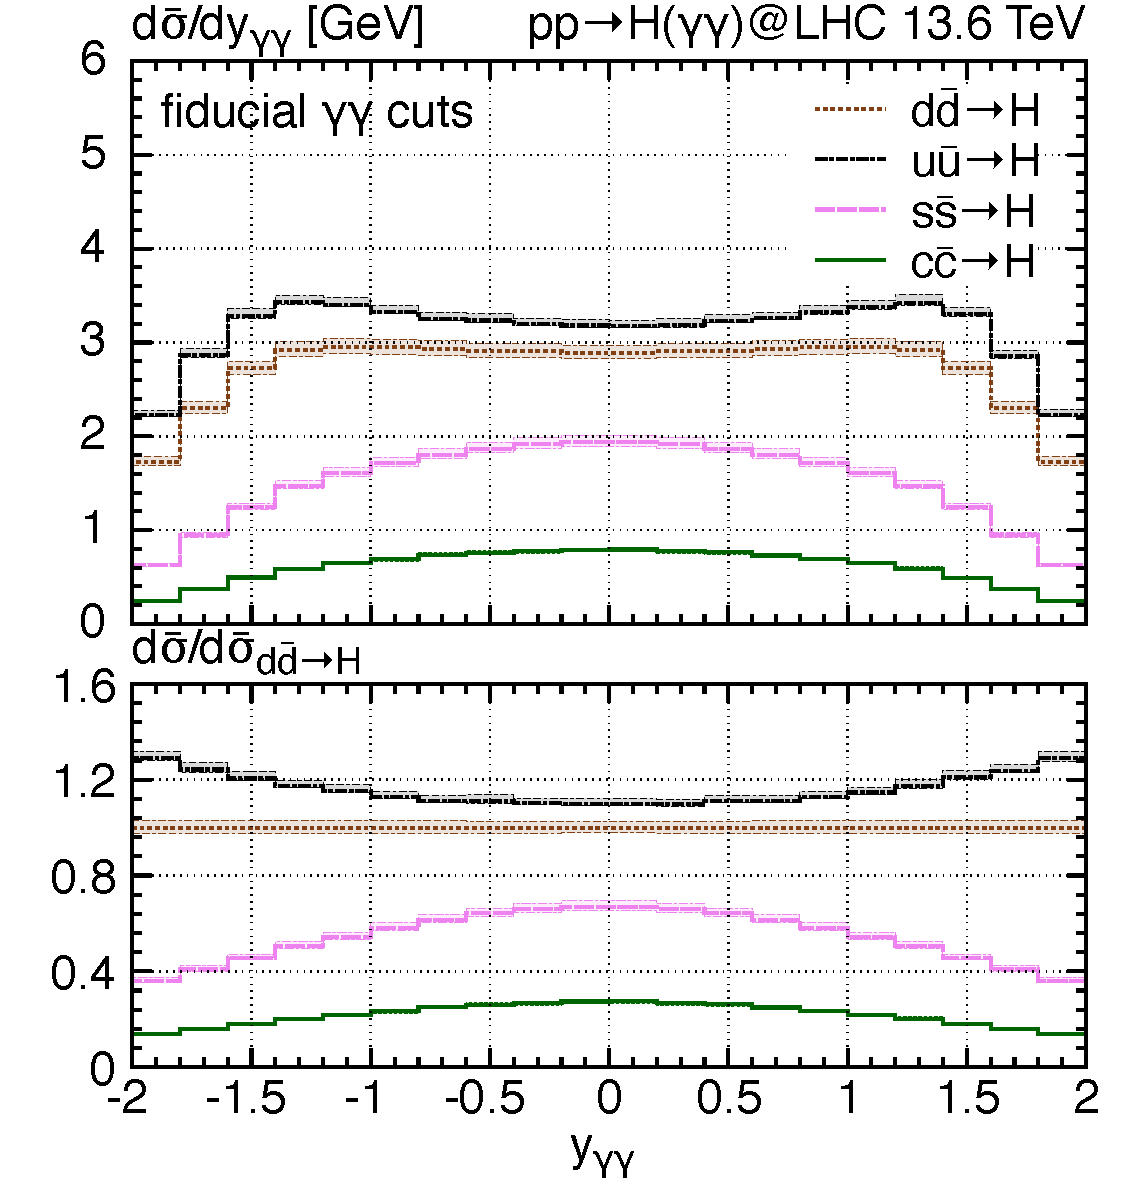
\includegraphics[width=.45\textwidth, page=1]{plots/5fs/light/y_Higgs-aafid.pdf}
\end{tabular}
\vspace*{1ex}
\caption{Rapidity distribution of the hardest photon in the fully inclusive setup (left) and of the reconstructed Higgs boson in the fiducial region (right), for light-parton fusion initiated by up- (black, short-dashed), down- (brown, dotted), strange- (pink, long-dashed), and charm-quarks (blue, solid).\label{fig:lightrapidity}}
\end{center}
\end{figure}

We now present a selection of differential results. The shape of the Higgs transverse momentum spectrum for quark-initiated processes differs significantly from that in the gluon-initiated channel, offering a clearer possibility to study the interaction between the Higgs boson and partons. In the first plot of figure~\ref{fig:lightpTH}, we show the transverse momentum spectrum of the Higgs boson, reconstructed from the diphoton pair in the fully inclusive setup. It displays similar shapes across the different flavour channels, with normalisation reflecting the corresponding total cross sections. The second plot in figure~\ref{fig:lightpTH} shows the same distribution, but for events where the photons pass the fiducial cuts. In this scenario, more pronounced differences in shape emerge among the various channels. In particular, the up-quark contribution—about 1.5 times larger than the down-quark prediction in the fully inclusive case because of PDF enhancement—has a strong reduction in the fiducial region. Indeed, at intermediate values of transverse momentum, the up- and down-quark channels yield comparable results when the same Yukawa strength is assumed. Moreover, once the relative mass suppression in the Yukawa couplings is taken into account, the up-quark prediction falls below the down-quark one.

The main origin of this effect is the rapidity constraint defined in~\eqn{eq:aafidmycuts}. Indeed, the parton distribution functions influence the photon rapidity shape, yielding distinctive behaviour in the up-quark channel. The first plot in figure~\ref{fig:lightrapidity} shows the rapidity distribution of the photon with the highest transverse momentum across the different channels; similar patterns are observed for the second photon. For strange- and charm-quark fusion, as well as for the bottom-quark case, the distribution peaks around zero rapidity. In contrast, valence quark channels exhibit different shapes due to their characteristic parton luminosities. The down-quark channel shows a plateau for $|y_\gamma| < 2$, whereas the up-quark channel features a distribution not centred around zero rapidity, with a significant fraction of the cross section residing at larger rapidity values. As a result, the cut $|y_\gamma| < 2.37$ has a more pronounced impact on the up-quark distribution, removing a larger portion of the cross section when applying the fiducial selection. We have confirmed a similar trend at leading order, with a shape validated using the mass-rapidity scan of PDF4LHC luminosities obtained using \texttt{APFEL}~\cite{Bertone:2013vaa}. This distinctive behaviour, more evident here than in neutral Drell–Yan due to the higher Higgs mass, provides a useful handle for differential studies, as the rapidity spectrum in light-quark fusion differs markedly from dominant production modes. We conclude by presenting the Higgs boson rapidity, reconstructed from the two photons that satisfy the fiducial cuts~\eqref{eq:aafidmycuts}, as shown in the second plot of figure~\ref{fig:lightrapidity}. In the exclusive region, the up-quark behaviour is more similar to the down-quark, with a cross section between 1.1 and 1.3 times that of the down-quark process. The charm-quark and the strange-quark exhibit a steeper distribution compared to the Higgs boson from down-quark fusion.

In this section, we have presented the NNLO+PS generator for Higgs production via light-parton fusion with decay into photons as a potential tool to constrain light-quark Yukawa couplings. We conclude by noting that alternative channels sensitive to light-quark Yukawa couplings have been experimentally investigated recently, such as the Higgs decay rate into four leptons~\cite{CMS:2025xkn}.
\section{Outlooks and Conclusions}

\textbf{Citation policy. }\\

\textbf{Acknowledgements. }CB is grateful to Tommaso Giani for PDF insights and Jan Lukas Spah for interesting discussions on Yukawa interactions via light-quark fusion. We have used the Max Planck Computing and Data Facility (MPCDF) in Garching to carry out the \minnlo{} simulations presented here for \bbtoH{}, $q\bar q\rightarrow \text{H}$ and \bbH{} production.

\bibliography{bbh}
\bibliographystyle{JHEP}

\end{document}
